%%%%%%%%%%%%%%%%%%%%%%%%%%%%%%%%%%%%%%%%%
% Thesis Proposal
%
% Francesc Wilhelmi Roca
% Boris Bellala, Cristina Cano, Anders Jonsson
% Wireless Networking Research Group
% Universitat Pompeu Fabra
%%%%%%%%%%%%%%%%%%%%%%%%%%%%%%%%%%%%%%%%%

\documentclass[12pt, a4paper,twoside]{tesi_upf}
%\usepackage[latin1]{inputenc}
\usepackage[catalan,english]{babel}
\usepackage[cam,a4,center,frame]{crop}
\usepackage{graphicx}
\usepackage{times}
\usepackage{makeidx}
\usepackage{url}
\usepackage{subcaption}

%% Tikz libraries
\usepackage{tikz}
\usepackage{tkz-tab}
\usetikzlibrary{automata,arrows,positioning,calc}
\usetikzlibrary{shapes,snakes}

\usepackage[utf8]{inputenc}


\usepackage{color}
\usepackage{amsmath}
\usepackage{mathtools}
\usepackage{fullpage}
\usepackage{algorithmic}
\DeclareMathOperator*{\argmin}{argmin}
\algsetup{linenosize=\small}
%\usepackage[table,xcdraw]{xcolor}
\usepackage{multirow}
\usepackage[super]{nth}
\usepackage{graphicx}
\usepackage{caption}
\usepackage[labelformat=simple]{subcaption}
\usepackage{setspace}
\usepackage{textcomp}
\usepackage{xspace}
\usepackage{siunitx}
\usepackage{epsfig}
\usepackage{epstopdf}
\usepackage{soul}
\usepackage{url}
\usepackage{tablefootnote}
\DeclareMathOperator{\E}{\mathbb{E}} % Expectation Symbol
\usepackage[linesnumbered,ruled]{algorithm2e}
\usepackage{booktabs}
\usepackage{pgfgantt}
\usepackage[catalan,english]{babel}
\pagestyle{plain}
\selectlanguage{english}

\title{Reinforcement Learning to Enhance Spatial Reuse in Dense Wireless Networks}
\author{Francesc Wilhelmi}
\supervisor{Boris Bellalta, Cristina Cano \& Anders Jonsson}
\department{Department of Information and Communication Technologies\\
	Universitat Pompeu Fabra, Barcelona}
\thyear{September 2017}

\begin{document}

	\frontmatter
	
	\maketitle
	
	\cleardoublepage
	
	\selectlanguage{english}
	
	\mainmatter
	
	\tableofcontents
	
	%%%%%%%%%%%%%%%%%%%%%%%%%%%%%%%%%%%%%%%
	% INTRODUCTION       								   %%%%%%%%%%%%%
	%%%%%%%%%%%%%%%%%%%%%%%%%%%%%%%%%%%%%%%
	\chapter{Motivation}
	\label{section:introduction}	
		Due to the growing popularity of wireless deployments (especially the ones based in the IEEE 802.11 standard), it is very common to find overlapping Wireless Networks (WNs) that squander the bandwidth resources. This is mostly provoked by a lack of organization and/or agreement at sharing it, and the problem scales up as the number of overlapping nodes increases. A prominent example about the harmfulness of such type of coexistence is that the default power level of devices in a WN is typically set to the maximum, regardless of the distance between nodes and the channel occupancy \cite{akella2007self}. Moreover, according to \cite{zhong2015issues}, the network performance is severely deteriorated as density increases, specially if the number of Overlapping Basic Service Sets (OBSSs) is greater than 1. If we consider dense scenarios such as stadiums, trains or apartment buildings, then the combination of bad performance and high density entails to provide challenging solutions. For that, the IEEE 802.11ax-2019 standard is being developed by the Task Group AX (TGax). The standard emphasises on spatial reuse to fulfil , in addition to include many other novel mechanisms such as Orthogonal Frequency-Division Multiple Access (OFDMA), Dynamic Channel Bonding (DCB), and Multi-User Multiple Input Multiple Output (MU-MIMO). Spatial reuse aims to reduce the interference level in an overlapping scenario, so that the area throughput can be maximised. To enhance spatial reuse, we highlight Transmission Power Control (TPC), Carrier Sense Threshold (CST) adjustment, and beamforming. 
		
		In addition to the coexistence issues (further described in Section \ref{section:coexistence_issues}) resulting from new requirements, the variability in wireless networks in terms of user arrivals and departures entails another challenge to the resource allocation problem. Thus, adaptable and fast-convergence solutions must be provided, which even increases their complexity. Henceforth, the dynamic adjustment of parameters such as the frequency channel, the transmit power, or the sensitivity, appears to suit properly in the Reinforcement Learning (RL) paradigm. In RL, input signals are used to determine the behaviour of a given system, so that historical events are considered for decision-making. To validate a real-time solution, it is very important to build an accurate model that takes into account the users behaviour. Thus, considering arrivals and departures is key for designing a solution, which is required to be provided before the environment changes. In both \cite{balachandran2002characterizing} and \cite{papadopouli2005modeling}, user arrivals are modelled as time-varying Poisson processes, such that the users arrival rate ($\lambda$) depends on the time. On these works, it is studied the users' behaviour in fully controlled environments such as University Campus or Conferences, but the mean time between user arrivals varies according to the scenario and many other factors. In particular, in the second case it is considered a two-state Markov-Modulated Poisson Process (MMPP) with mean inter-arrival times of 38 seconds and 6 minutes for accessing and leaving the system, respectively, which provides us a first idea about the maximum allowed convergence time for the developed solutions. In addition to scenarios diversification, it should be considered what will be the users behaviour in the future, as well as the algorithms to be designed must operate in the long term. 
		
		\section{Document Structure}
			The remainder of this documents is structured as follows: Section \ref{section:research_problem} presents the Research Problem, as well as open challenges regarding the spatial reuse problem in WNs. The related work is shown in Section \ref{section:state_of_the_art}, as well as the current literature in the application of Reinforcement Learning (RL) to Wireless Communications. Then, Section \ref{section:contributions} presents the ongoing work and the current contributions. Finally, the working plan and the expected goals are provided in Section \ref{section:future_work}.

	%%%%%%%%%%%%%%%%%%%%%%%%%%%%%%%%%%%%%%%
	% RESEARCH PROBLEM							      %%%%%%%%%%%%%
	%%%%%%%%%%%%%%%%%%%%%%%%%%%%%%%%%%%%%%%
	\chapter{Research Problem}
	\label{section:research_problem}
		In this Section we describe the current issues and open challenges for the spatial reuse problem in overlapping WNs. Note that IEEE 802.11 Wireless Local Area Networks (WLANs) are particularly focused to narrow the problem characterisation.
		
		%%%%%%%%%%%%%%%%%%%%%%%%%%%%%%%%%%%%%%%
		% COEXISTENCE ISSUES						      %%%%%%%%%%%%%
		%%%%%%%%%%%%%%%%%%%%%%%%%%%%%%%%%%%%%%%
		\section{Coexistence Issues in IEEE 802.11 WLANs}
		\label{section:coexistence_issues}	
			IEEE 802.11 WLANs implement Distributed Coordination Function (DCF) for dealing with coexistence, which is based on a combination of Carrier Sense Multiple Access with Collision Avoidance (CSMA/CA) and Binary Exponential Backoff (BEB) protocols. It basically consists on letting stations listen to the channel for a period called Distributed Inter Frame Space (DIFS) before transmitting, in order to ensure that the channel is going to be clear when sending information over it. Channel is sensed to be free according to the Clear Channel Assessment (CCA) mechanism, i.e., if the power sensed is lower than a given threshold. The power received at a given node is the sum of all the interferences generated by the other devices under the environment-constrained propagation effects. Regarding BEB, the aim is to reduce the number of potential collisions by randomizing the access to the channel and adapting the opportunities for accessing to it. In BEB, each station selects a random backoff value to start a countdown that prevents to transmit until it has been exhausted, thus minimizing collisions. In case channel is sensed as busy, the countdown is paused and resumed as soon as the ongoing transmission finishes. Note that the backoff is a uniformly distributed random variable between 0 and the Contention Window (CW), which is doubled in case of noticing a packet failure until reaching a maximum value $\text{CW}_{max}$. The probability of noticing a collision decreases as CW increases, but this supposes that channel is free more time, which also harms the overall throughput.
					
			Despite of the mechanisms implemented at IEEE 802.11 WLANs and due to the nature of the CSMA/CA protocol, coexistence still drives into many problems and situations such as the hidden or the exposed terminal problems. It exists a trade-off between the collisions occurring in a OBSS, the time channel remains idle, and the overhead generated to avoid harmful situations. In all the cases both throughput and fairness of the coexisting networks are compromised and it is required to find a solution that better performs on each situation.	The Exposed-Terminal problem (or exposed node problem) occurs when a device is prevented to transmit due to the sensed interferences caused by other nodes, so that the CCA threshold that considers the channel as busy is exceeded. Thus, throughput is reduced according to the number of exposed nodes that are sharing the same channel. On the other hand, the Hidden-Terminal node may generate collisions if two out-of-range nodes transmit at the same time to a node that senses both. In this case, the performance is affected by a higher collision probability, which may entail severe issues at several levels of the network architecture such as routing or transport. Figure \ref{fig:hidden_exposed} shows both Hidden and Exposed Terminal Problems.					
			\begin{figure}[h!]
				\centering
				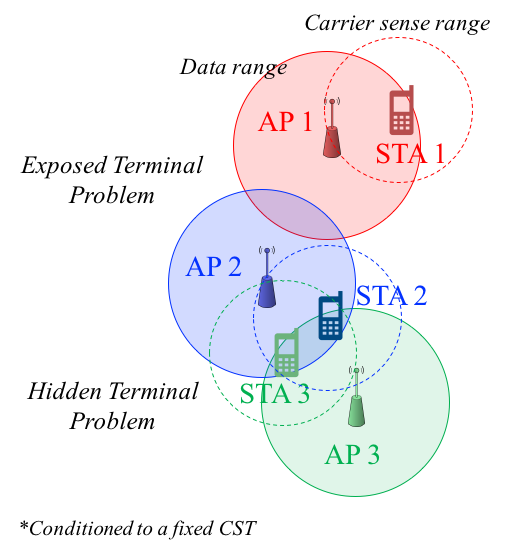
\epsfig{file=images/hidden_exposed.png, width=10cm}
				\caption{Exposed Terminal Problem: AP1 and AP2 could transmit simultaneously since STA1 and STA2 are enough away from the interference, but only a transmission at a time is allowed due to CSMA/CA. Hidden Terminal Problem: AP2 and AP3 may suffer collisions by hidden node because they are not in range each other, but STA2 and STA3 do.}
				\label{fig:hidden_exposed}
			\end{figure}		
			
			In order to minimise the hidden-terminal problem, the IEEE 802.11 amendment includes the optional Request-to-Send / Clear-to-Send (RTS/CTS) mechanism. It basically consists in pre-allocating the channel before performing a data transmission. To do so, both source and destination interchange RTS and CTS frames in case the channel is sensed as free from both locations. Thus, potential hidden nodes go into a virtual carrier-sensing mode in case of listening any of the two frames. The Network Allocation Vector (NAV) is responsible to handle this virtual sensing. Figure \ref{fig:dcf_operation} shows the DCF operation with RTS/CTS.					
			\begin{figure}[h!]
				\centering
				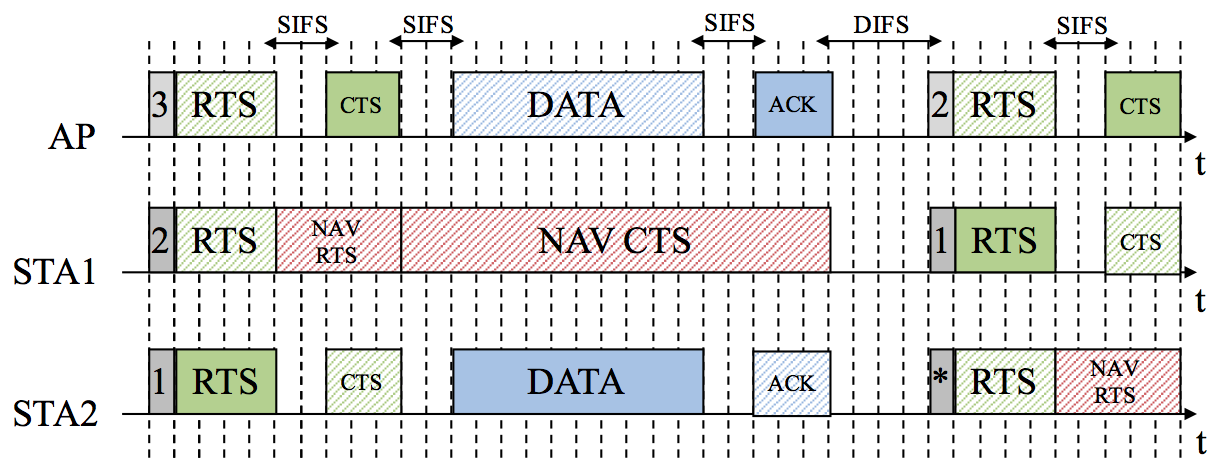
\epsfig{file=images/dcf_operation.png, width=12cm}
				\caption{DCF operation with RTS/CTS. After waiting 1 slot, STA2 sends an RTS frame to indicate that it wants to reserve the channel. A CTS frame is replied from the AP, so NAV is updated in STA1 to cover the entire transmission, as well as it operates at the same frequency channel.}
				\label{fig:dcf_operation}
			\end{figure}
		
			However, RTS/CTS can fail at solving the hidden-terminal problem, since either RTS and CTS frames may be not heard by interfering nodes, and some other counter productive effects are well-known to occur \cite{sobrinho2005rts}. This is specially likely to occur in case of asymmetric links, which can be caused by using different transmit powers and carrier sense thresholds.
					
		%%%%%%%%%%%%%%%%%%%%%%%%%%%%%%%%%%%%%%%
		% SCENARIOS												   %%%%%%%%%%%%%
		%%%%%%%%%%%%%%%%%%%%%%%%%%%%%%%%%%%%%%%						
		\section{Scenarios}
		\label{section:scenarios}	
		According to \cite{bellalta2016ieee}, next-generation WLANs will lead to dense scenarios, containing a high number of wireless devices (e.g. 1 user/m$^2$). Typical dense scenarios are provided by the IEEE 802.11ax amendment:
		\begin{itemize}			
			\item \textbf{Residential Scenario:} this scenario aims to characterise a typical uncoordinated deployment of WLANs, combining HEW and legacy devices. It consists in a 5-floors building of 3 m per floor (see Figure \ref{fig:building}), containing 2x10 apartments, which have size 10m x 10m x 3m (see Figure \ref{fig:floor}). An indoor path-loss model is used to capture the effect of walls and other obstacles on the propagated signals. 
			\begin{figure}[h!]
				\centering
				\begin{subfigure}[b]{0.4\textwidth}
					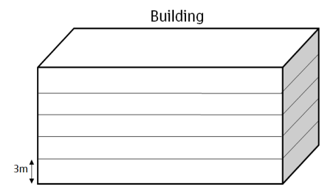
\includegraphics[width=\textwidth]{images/residential_ax_1}
					\caption{Building layout}
					\label{fig:building}
				\end{subfigure}
				\begin{subfigure}[b]{0.4\textwidth}
					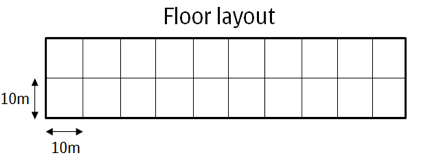
\includegraphics[width=\textwidth]{images/residential_ax_2}
					\caption{Floor layout}
					\label{fig:floor}
				\end{subfigure}		
				\caption{IEEE 802.11ax Residential scenario}
				\label{fig:ax_residential_scenario}
			\end{figure}			
			\item \textbf{Enterprise Scenario:} in this case, it is presented a coordinated scenario in which devices are mostly controlled. It is composed by 8 offices (see Figure \ref{fig:offices}), containing 64 cubicles (see Figure \ref{fig:cubicles}). In office there are 4 APs installed in a mesh topology, and in each cubicle there are 4 STAs (laptop, monitor, smartphone or tablet, and hard disk). The interferences generated in such scenario are the ones provided by the overlapping ESSs and unmanaged networks (P2P links). The path-loss considered takes into account the walls of the offices.
			\begin{figure}[t!]
				\centering
				\begin{subfigure}[b]{0.4\textwidth}
					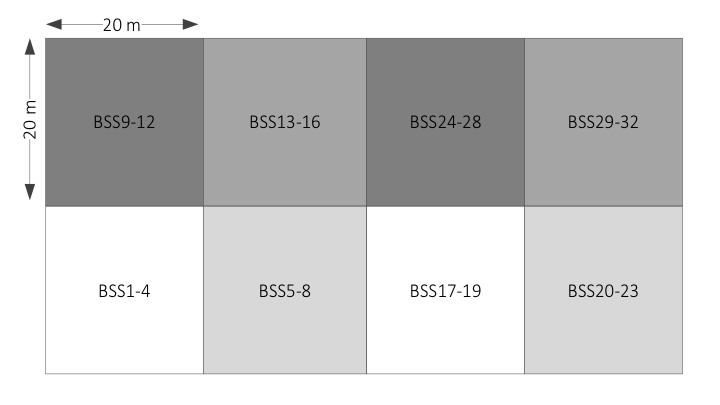
\includegraphics[width=\textwidth]{images/enterprise_ax_1}
					\caption{Offices layout}
					\label{fig:offices}
				\end{subfigure}
				\begin{subfigure}[b]{0.4\textwidth}
					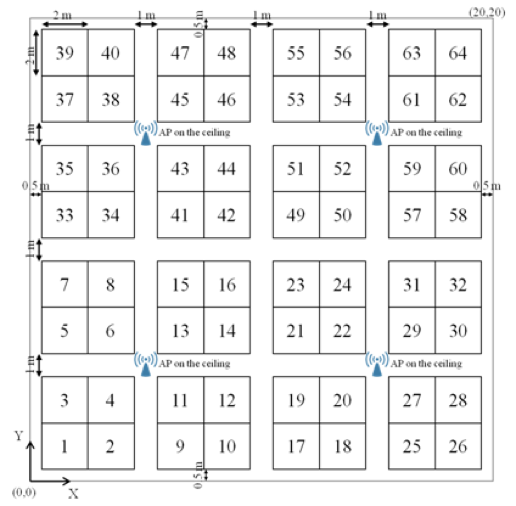
\includegraphics[width=\textwidth]{images/enterprise_ax_2}
					\caption{Cubicles layout}
					\label{fig:cubicles}
				\end{subfigure}		
				\caption{IEEE 802.11ax Enterprise scenario}
				\label{fig:ax_enterprise_scenario}
			\end{figure}
		
			\item \textbf{Indoor Small BSS  Scenario:} this scenario aims to represent coordinated real-world deployments that aim to extend mobile networks to support a high number STAs by placing many long-range APs. The ESS architecture is therefore planned through a given frequency reuse pattern (see Figure \ref{fig:large_ax}). The radius of each cell has size 10 m, and there are $2 \cdot h$ meters between consecutive BSSs, where $h=sqrt(R2-R2/4)$. The AP is placed at the centre of the cell.			

			\item \textbf{Outdoor Large BSS Scenario:} similarly to the indoor BSS scenario, the objective for the outdoor large BSS scenario is to capture issues in real-world outdoor deployments with a high separation between BSSs. Again, the deployment is planned, so as the frequency reuse. The scenario is composed by 19 hexagonal grids, with an inter-AP separation of 130m. STAs are placed randomly through a uniform distribution, so that they associate to the nearest AP based on distance-based path loss and shadowing.  
			\begin{figure}[h!]
				\centering
				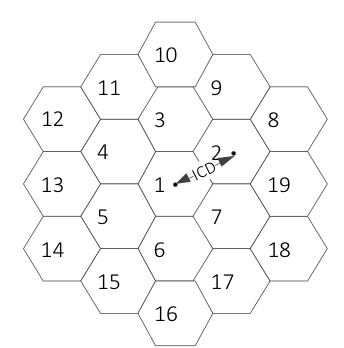
\epsfig{file=images/large_ax.png, width=5cm}
				\caption{IEEE 802.11ax Cell topologies}
				\label{fig:large_ax}
			\end{figure}	
		
			\item \textbf{Residential Scenario + Outdoor Large BSS Scenario:} it is a combination of the residential and the outdoor scenarios, so that different path-loss models are considered due to walls penetration in the building case.
			\begin{figure}[h!]
				\centering
				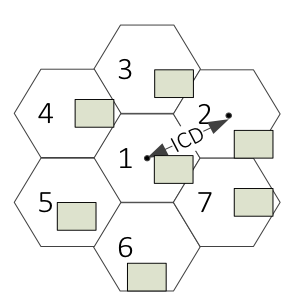
\epsfig{file=images/residential_large_ax.png, width=5cm}
				\caption{IEEE 802.11ax Residential + Large Outdoor BSS scenario}
				\label{fig:residential_large_ax}
			\end{figure}	
		\end{itemize}
			
		%%%%%%%%%%%%%%%%%%%%%%%%%%%%%%%%%%%%%%%
		% SPATIAL REUSE										     %%%%%%%%%%%%%
		%%%%%%%%%%%%%%%%%%%%%%%%%%%%%%%%%%%%%%%			
		\section{Spatial Reuse in Overlapping IEEE 802.11 WLANs}
		\label{section:spatial_reuse}		
			To deal with the aforementioned problems caused by coexistence, spatial reuse turns out to be key, so as to improve the area throughput. The first step to enhance spatial reuse is to properly allocate frequency channels among coexisting nodes, so that interference is minimised. Due to the traffic and users fluctuation, Dynamic Channel Allocation (DCA) is required to maximise the performance of the wireless networks in dense environments. DCA aims to properly allocate the available frequency range among the overlapping devices. Several approaches can be found for DCA according to the needs, and there is a strong discussion about which requirements must be accomplished. While some approaches aim to provide fairness (\cite{ling2006joint}), some others try to grant more resources to nodes with higher traffic demands (\cite{wertz2004automatic}). 
			
			Another mechanism of interest to improve spatial reuse is Transmission Power Control (TPC), which can also help at reducing energy consumption. By adjusting the transmit power, the number of exposed nodes can be minimised, allowing a higher number of parallel transmissions within the same range. But there is an important consideration at tuning the power transmitted, which is that data rate directly depends on the SINR sensed at the receiver (the less power transmitted, the less experienced data rate received). Thus, adjusting TPC poses the trade-off between the number of parallel transmissions and the quality of them. Moreover, an insufficient transmit power may be unheard at the receiver, leading into packet losses. 
			
			Finally, Carrier Sense Threshold (CST) adjustment may also help to increase the number of parallel transmissions and minimizing the collisions probability by hidden-node. However, modifying the CST entails several consequences. For instance, decreasing the CST may rise probability of finding hidden nodes (the less is listened, the less is known). Table \ref{tbl:cca_tpc_effects} summarises the effects of TPC and CST adaptation.			
			\begin{table}[h!]
				\centering
				\begin{tabular}{|c|c|c|c|c|}
					\hline
					\multirow{2}{*}{\begin{tabular}[c]{@{}c@{}}\\ \textbf{Action}\end{tabular}} & \multicolumn{4}{|c|}{\textbf{Effect}} \\ \cline{2-5} 
					& \begin{tabular}[c]{@{}c@{}}Parallel\\ Transmissions\end{tabular}  & Data Rate & \begin{tabular}[c]{@{}c@{}}Collisions probability\\ (by hidden node)\end{tabular} & \begin{tabular}[c]{@{}c@{}}Energy\\ Consumption\end{tabular}\\ \hline
					$\uparrow$ Power & $\downarrow$ & $\uparrow$ & $\downarrow$ & $\uparrow$ \\ \hline
					$\downarrow$ Power & $\uparrow$ & $\downarrow$ & $\uparrow$ & $\downarrow$ \\ \hline
					$\uparrow$ CCA & $\downarrow$ & - & $\downarrow$ & $\downarrow$* \\ \hline
					$\downarrow$ CCA & $\uparrow$ & - & $\uparrow$ & $\uparrow$* \\ \hline
				\end{tabular}
				\caption{Effects of TPC and CST adjustment. \textit{*Adjusting CCA may indirectly affect to the energy consumption by requiring more/less power to be transmitted.}}
				\label{tbl:cca_tpc_effects}
			\end{table}
			
			The modification of channel, transmit power and CCA may provide enormous enhancements to spatial reuse, but finding the optimal solution for a given Wireless Network is NP-hard. For that, we put special emphasis on Reinforcement Learning (RL) for improving the spatial reuse. RL turns out to be a convenient paradigm for allowing independent devices to improve their own performance through an observations-based learning process. Therefore, the main concern of this work is to let WNs to self-adjust both frequency channel and transmit power through a learning approach that uses only local information. On one hand, this allows avoiding the extra overhead that may be generated by the communication between WNs (which may be counter productive in terms of throughput). On the other hand, learning in WNs using only local information presents a number of challenges that must be faced in order to approach the resource allocation problem, which is also of relevance for this work.		

	%%%%%%%%%%%%%%%%%%%%%%%%%%%%%%%%%%%%%%%
	% STATE OF THE ART				                 %%%%%%%%%%%%%
	%%%%%%%%%%%%%%%%%%%%%%%%%%%%%%%%%%%%%%%	
	\chapter{State of the Art}
	\label{section:state_of_the_art}
		This Section describes the previous related work to enhance spatial reuse in Wireless Networks regarding channel, transmit power and sensitivity adjustment. Furthermore, it introduces previous research in dynamic resource allocation in WNs through Reinforcement Learning.		
			
		%%%%%%%%%%%%%%%%%%%%%%%%%%%%%%%%%%%%%%%
		% SoA DCA										          %%%%%%%%%%%%%
		%%%%%%%%%%%%%%%%%%%%%%%%%%%%%%%%%%%%%%%				
		\section{Dynamic Channel Allocation}		
		\label{section:dca}
			The Industrial, Scientific and Medical (ISM) band is shared by multiple technologies such as IEEE 802.11, IEEE 802.15 and Unlicensed Long Term Evolution (U-LTE). In particular, most of the Wi-Fi standards use the 2.4 GHz	and 5 GHz bands, which have different number of channels. For the 2.4 GHz case, there are 14 overlapping channels of 22 MHz (refer to Figure \ref{fig:channelisation_wifi}), so that adjacent channel utilisation ($\pm$ 11 MHz) is affected by a 30 dB signal drop (shown in Figure \ref{fig:80211ad_mask}). Similarly, the 5 GHz band is composed by three subbands, each one containing four non-overlapping channels. For using this band it is required to implement some mechanisms such as Dynamic Frequency Selection (DFS) or Transmit Power Control (TPC).
			\begin{figure}[h!]
				\centering
				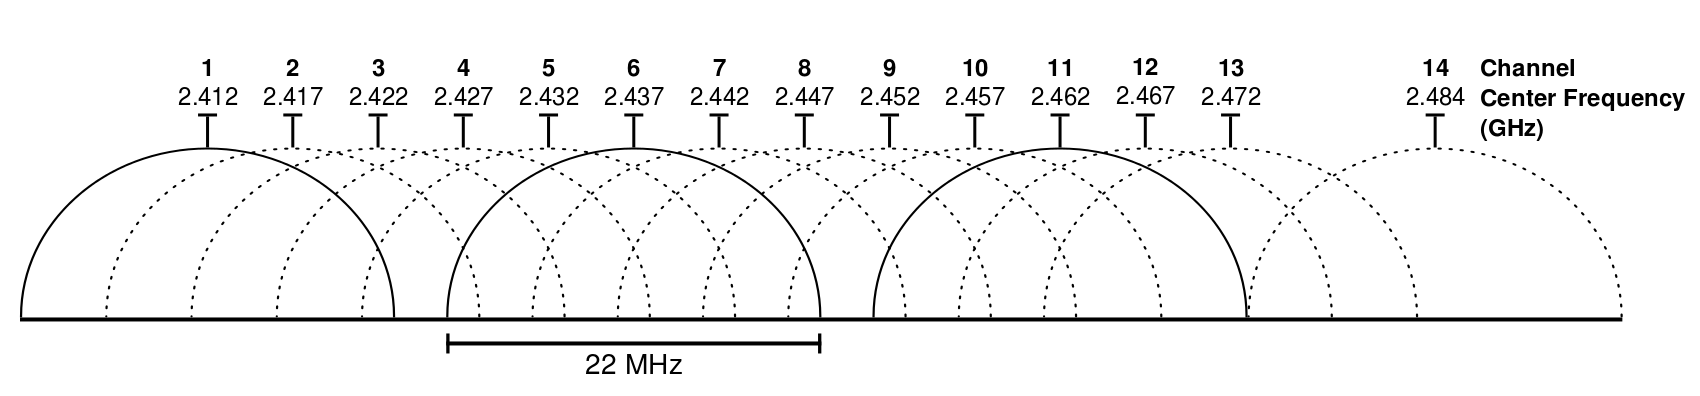
\epsfig{file=images/channelisation_wifi.png, width=15cm}
				\caption{Channelisation of the 2.4 GHz band}
				\label{fig:channelisation_wifi}
			\end{figure}
			\begin{figure}[h!]
				\centering
				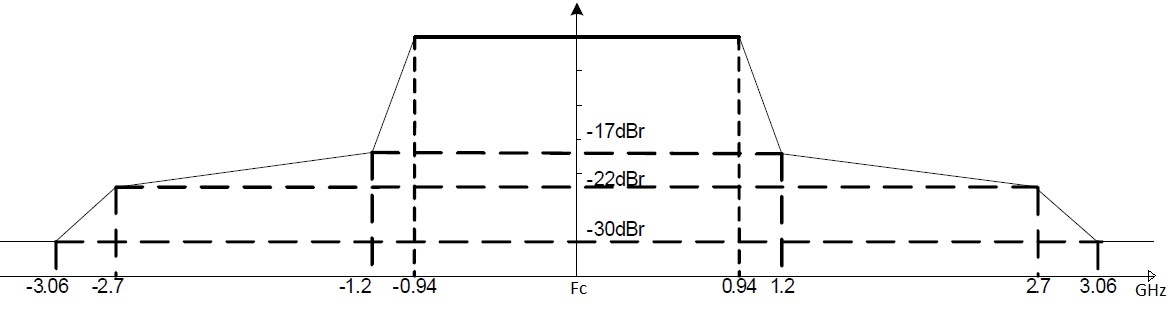
\epsfig{file=images/WLAN-802-11-spectrum-mask.jpg, width=11cm}
				\caption{IEEE 802.11 mask}
				\label{fig:80211ad_mask}
			\end{figure}
			
			The saturation of the unlicensed bands requires a proper channel allocation, which for dense deployments becomes a challenging task due to the scarce number of available non-overlapping channels. Thus, both frequency planning and dynamic channel selection have been of remarkable interest to the wireless communications community for enhancing the throughput area in overlapping WNs. A proper frequency planning allows reducing the interference between wireless devices, thus enhancing the overlapping networks capacity by avoiding collisions and delayed medium accesses. Dynamic channel selection allows wireless devices to change their centre frequency according to channel utilisation, which depends on the surrounding environment. A survey of channel assignment is provided in \cite{chieochan2010channel}, which introduced techniques are summarised in Tables \ref{tbl:channel_assignment_coordinated} and \ref{tbl:channel_assignment_uncoordinated}.
			
			\begin{table}[]
				\centering
				\begin{tabular}{llcc}
					\hline
					\multicolumn{1}{c}{\textbf{Technique}} & \multicolumn{1}{c}{\textbf{Description}} & \textbf{References} & \textbf{\begin{tabular}[c]{@{}c@{}}With AP \\ Placement\end{tabular}} \\ 
					\hline
					\begin{tabular}[c]{@{}l@{}}Graph \\ Colouring\end{tabular} & \begin{tabular}[c]{@{}l@{}}By assuming that APs are vertexes \\ and non-overlapping channels are\\ colours, graph colouring is applied to\\ minimise the interference between\\ adjacent cells. Graph colouring can be\\ also used for AP placement.\end{tabular} & \cite{hills2001large,mahonen2004automatic, riihijarvi2005frequency,riihijarvi2006performance} & Yes / No \\ \hline
					\begin{tabular}[c]{@{}l@{}}Integer Linear \\ Programming \\ (ILP)\end{tabular} & \begin{tabular}[c]{@{}l@{}}ILP is used to place APs and assign \\ channels by considering load balancing.\end{tabular} & \cite{lee2002optimization} & Yes \\ \hline
					\begin{tabular}[c]{@{}l@{}}Priority-Map \\ Approach\end{tabular} & \begin{tabular}[c]{@{}l@{}}A floor plan is divided into pixels, \\ which are assigned different priorities.\\ Then, both channel assignment and\\ AP placement is solved according to\\ built priorities.\end{tabular} & \cite{wertz2004automatic} & Yes \\ \hline
					\begin{tabular}[c]{@{}l@{}}Patching \\ Algorithm\end{tabular} & \begin{tabular}[c]{@{}l@{}}An heuristic algorithm is proposed\\ for maximising the throughput\\ and the fairness among wireless \\ clients, so that APs are being \\ sequentially placed according to \\ an objective function.\end{tabular} & \cite{ling2006joint} & Yes \\ \hline
					\begin{tabular}[c]{@{}l@{}}Coverage-\\ Oriented \\ Approach\end{tabular} & \begin{tabular}[c]{@{}l@{}}Linear programming is used to \\ optimise channel assignment and\\ AP placement, so that two objective\\ functions are used to that purposes.\end{tabular} & \cite{eisenblatter2007integrated} & Yes \\ \hline
					\begin{tabular}[c]{@{}l@{}}Conflict-free\\ Set Colouring\end{tabular} & \begin{tabular}[c]{@{}l@{}}Optimal AP association is provided \\ to minimise the interference\end{tabular} & \cite{mishra2006client} & No \\ \hline
					\begin{tabular}[c]{@{}l@{}}Measurement-\\ based local \\ coordination\end{tabular} & \begin{tabular}[c]{@{}l@{}}Both APs and clients need to measure\\ the interference sensed in all the \\ frequency channels in order to derive\\ an optimal solution for channel\\ assignment.\end{tabular} & \cite{chen2007improved} & No\\ \hline
				\end{tabular}
				\caption{Coordinated approaches for channel assignment}
				\label{tbl:channel_assignment_coordinated}
			\end{table}
			
			\begin{table}[]
				\centering
				\begin{tabular}{llc}
					\hline
					\multicolumn{1}{c}{\textbf{Technique}} & \multicolumn{1}{c}{\textbf{Description}} & \textbf{References} \\ \hline
					\begin{tabular}[c]{@{}l@{}}Least Congested\\ Channel Search\\ (LCCS)\end{tabular} & \begin{tabular}[c]{@{}l@{}}APs listen to all the channels and select\\ the one with lowest sensed interference.\\ Other parameters such as traffic \\ information is also used to make a \\ decision.\end{tabular} & \cite{achanta2004method} \\ \hline
					\begin{tabular}[c]{@{}l@{}}MinMax\\ Approaches\end{tabular} & \begin{tabular}[c]{@{}l@{}}Based on the assumption that heavily\\ loaded APs degradate the network\\ performance, MinMax aims to minimise\\ the maximum effective channel \\ utilisation of those devices.\end{tabular} & \cite{leung2003frequency,yu2006dynamic,yu2004adaptive} \\ \hline
					\begin{tabular}[c]{@{}l@{}}Weighted\\ Colouring\end{tabular} & \begin{tabular}[c]{@{}l@{}}From the devices' perspective, it is \\ used the sensed interference and the \\ number of overlapping devices to \\ minimise an objective function that leads\\ to channel assignment.\end{tabular} & \cite{mishra2005weighted} \\ \hline
					\begin{tabular}[c]{@{}l@{}}Pick-rand and\\ Pick-first\end{tabular} & \begin{tabular}[c]{@{}l@{}}Based on the sensed interference, a new\\ channel is chosen randomly or according\\ to a ranking list (based also on the power\\ sensed).\end{tabular} & \cite{akl2007dynamic,haidar2007channel, al2007enhanced}\\ \hline
					\begin{tabular}[c]{@{}l@{}}Channel\\ Hopping\end{tabular} & \begin{tabular}[c]{@{}l@{}}APs change their channel periodically in\\ order to maximise the throughput in a\\ long run.\end{tabular} & \cite{mishra2006distributed} \\ \hline
				\end{tabular}
				\caption{Uncoordinated approaches for channel assignment}
				\label{tbl:channel_assignment_uncoordinated}
			\end{table}
			
			Many of the reviewed techniques imply the existence of a central node that makes the channel assignment, which is infeasible for uncoordinated WNs such as in residential scenarios. In contrast, decentralised mechanisms allow dynamic channel allocation based only on local information. However, many of them require from inter-AP communication and may lead to non-optimal solutions.
		
			Centralised approaches allow to effectively provide optimal (or close-to-optimal) solutions to the channel assignment problem, since complete knowledge and control on the network is granted. Moreover, in \cite{baid2015understanding} it is shown that centralised approaches allow to significantly improve the performance of a network, even with the existence of independent devices. To make centralised channel allocation, the first related literature that we find is based in graph colouring techniques. In contrast, even if centralised approaches are used, graph colouring is an NP-hard problem, which makes from it an infeasible solution for large scale scenarios. To solve that, we find several works that use heuristics in practical applications. The authors in \cite{brelaz1979new} firstly introduced the DSATUR algorithm for that purpose, which models the frequency allocation problem using interference graphs, so that higher-degree nodes have preference at choosing their centre frequency. An extension of DSATUR is found in \cite{villegas2009frequency}, which includes packet losses and co-channel interference in the decision-making process. In this case, the degree of a node is not given by its connections, but also by the interference and the utilisation. Several architectures are provided for running the algorithm, but all of them entail a full communication between nodes, so centralisation is required. Another fully centralised approach is introduced by \cite{raniwala2004centralized} in the context of wireless mesh networks, showing improvements of factor 2.63 in real scenarios (wireless cards are used to run the channel assignment algorithm based on the load). To do so, the authors propose a load-aware algorithm for dynamic channel selection, so traffic information is required in before-hand to provide a new channels configuration. 
			
			As seen before, centralised approaches are very effective at maximising the network conditions at overlapping environments by providing a proper channel allocation. However, several limitations can be found in real world. Firstly, many overlapping wireless deployments are independent, so they cannot be managed by a central entity. In addition, the underlying communication required adds a higher degree of complexity, which solutions may lead to obtain counter productive overhead. For that, we aim to focus on decentralised approaches (with and without communication) that allow facing the channel allocation problem is a simple way in terms of synchronisation. For the cases at which communication is required, we are interested in quantifying the generated overhead in order to notice the actual improvements achieved. Regarding decentralised mechanisms for channel assignment, we first focus on \cite{mishra2005weighted}, which presents a weighted colouring approach to improve the resources sharing problem in overlapping WNs. In particular, two techniques are provided, which are a fully decentralised and a messaging passing techniques. Again, the channel assignment problem in WLANs is approached through graph colouring, providing edges to nodes that suffer from neighbouring interference. The goal is to assign colours (i.e., channels) to nodes, so that adjacent nodes use different channels, and at the same time their usage is minimised. The fact of experiencing co-channel interference makes from this a weighted colouring problem, so an objective function is provided. This function aims to minimise the interference suffered by devices in an overlapping network. To allow decentralisation, the algorithm can only attempt to minimise the interference of a given AP, which ends up to reducing the total interference if the network progressively adjusts itself as a whole. A step further to provide fast-convergence and better results in terms of interference, is to centralise the algorithm in order to consider the aggregate interference. For that, a reliable communication between APs must be carried out. Notwithstanding, the implication of this communication is not even mentioned in this work, so it is not possible to determine if the presented method is practical due to the overhead or even feasible.
			
			Furthermore, \cite{herzen2013distributed} shows that minimising the interference through an objective function is only worth for very dense scenarios, which lacks of flexibility at maximising the throughput area. To improve that, the authors present a fully decentralized approach through a minimisation function that takes into account the total sensed interference and a cost associated to the bandwidth utilisation. The sum of both measurements is referred as the \textit{energy}:
			\begin{equation}
			\mathcal{E} (\textbf{F},\textbf{B}) = \sum_{A \in \mathcal{A}} \sum_{B \in \mathcal{N}_A} I_A (B) + \sum_{A \in \mathcal{A}} cost_A (b_A)
			\end{equation}
			Where $I_A (B)$ is the interference sensed at BSS $A$, originated by the other WLANs $B \in \mathcal{N}_A$, and $cost_A (b_A)$ is the cost that BSS $A$ obtains from using bandwidth $b_A$. The algorithm works in the APs as follows:
			\begin{figure}[h!]
				\centering
				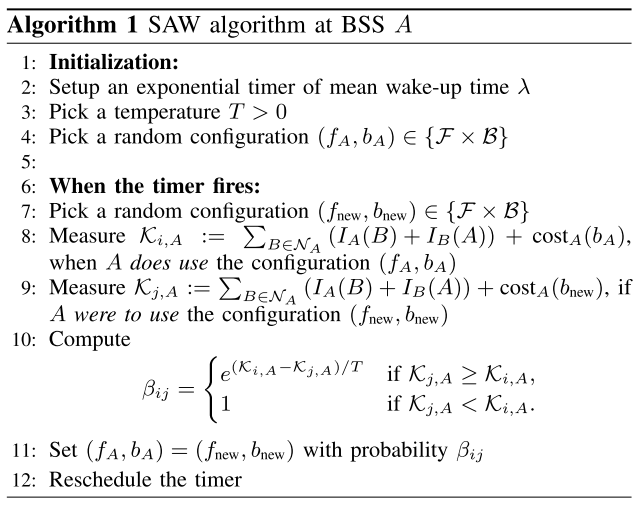
\epsfig{file=images/saw_alg.png, width=8cm}
				%\caption{}
				\label{fig:saw_alg}
			\end{figure}	
			The first experimental part (simulations carried out through Python) considers studying the modification of the cost function $c/b_A$ (where $c$ is a constant and $b_A$ is the bandwidth used by BSS $A$), so that different dynamics at the joint performance of the overlapping networks can be captured. For a null cost, the interference is attempted to be mitigated, which is shown to be effective for high densities. The opposite occurs for a larger value of $c$ (in this case, $c=100$), which is only useful to improve the capacity when few overlapping networks exist, but harms the overall performance in case density increases. In addition, fairness is shown to linearly decrease as $c$ increases. Then, a testbed implementation is provided by using 21 wireless nodes applying the channel allocation algorithm. It is shown a significant improvement for UDP and TCP traffic cases that overtakes the optimal performance achieved by applying frequency allocation through graph colouring.
								
			Other mechanisms for decentralised channel assignment that also rely in making measurements to enhance the network conditions can be found in \cite{akl2007dynamic, chen2007improved}. \cite{akl2007dynamic} proposes a very simple approach for letting the APs to maintain an interference map of their neighbours, such that channel assignment can be done through interference minimisation. Unfortunately, neither interactions between APs due to decentralisation are studied, nor strong evidences for improvements are provided. Separately, \cite{chen2007improved} proposes two decentralised approaches (in addition to a centralised one) that rely in the interference measured at both APs and STAs to calculate which are the best channels for dynamic channel allocation. An uncoordinated approach is shown, which presents acceptable results at minimising the interference in an overlapping network. In addition, a coordinated approach with messaging passing is presented, showing very good results. The main drawback is that the latter requires a wired infrastructure for the management communication, which is often infeasible, specially in typical residential scenarios. 				
			
			%%%%%%%%%%%%%%%%%%%%%%%%%%%%%%%%%%%%%%%
			% SoA TPC											      %%%%%%%%%%%%%
			%%%%%%%%%%%%%%%%%%%%%%%%%%%%%%%%%%%%%%%			
			\section{Previous Work in Transmit Power Control}
			\label{section:tpc}
				Adjusting the transmit power is another technique considered in the IEEE 802.11ax standard. In the first version of the draft \cite{tgax2016draft}, a set of regulations is provided for TPC usage. In particular, when a STA chooses a specific power detection level ($\text{OBSS\_PD}_{level}$), the maximum transmit power is given by:						
				\begin{scriptsize}
					\begin{equation}
					\text{TX\_PWR}_{max}=
					\begin{cases}
					\text{Unconstrained}, & \text{if}\ \text{OBSS\_PD}_{level} = \text{OBSS\_PD}_{min} \\
					\text{TX\_PWR}_{ref}-(\text{OBSS\_PD}_{level}-\text{OBSS\_PD}_{min}), & \text{OBSS\_PD}_{max} \geq \text{OBSS\_PD}_{level} \geq \text{OBSS\_PD}_{min}
					\end{cases}
					\nonumber
					\end{equation}				
				\end{scriptsize}
				
				Despite the context provided by the TGax, modifying the transmit power is a complex task that must be carefully done, since may affect to the higher communication layers such as network (routing) and transport (congestion). Since the transmission range and the data rate are conditioned by power control at the physical layer, the main effects of increasing the transmission power in a wireless network are:
				\begin{itemize}
					\item Generates more interference, which may cause a higher contention time for the overlapping nodes.
					\item Increases the data rate.
					\item Increases the transmission range, which is helpful for connectivity with the receiver but harmful for the overlapping nodes due to the generated interference.
					\item Increases the energy consumption.\footnote{Energy consumption is affected by the type of power consumption (power transmission, power idle, power sleep, power amplifier and power reception) and the devices involved in the communication. To apply a policy for saving power is strictly related to them, which is out of the scope of this Thesis.}
				\end{itemize}
				
				Furthermore, TPC may create unidirectional links, which unleashes fairness issues within overlapping nodes. In fact, acknowledgements (ACKs) and RTS/CTS frames assume bidirectional links. To properly implement TPC, the first question to be asked is where should power control be done in the network architecture. This question is presented in \cite{kawadia2005principles}, which, in addition to devising that the network level should be in charge of power control, presents a guideline of its impact on several performance measures (end to end delay, packet losses, routing overhead, etc.). The authors claim that global optimization is carried out by TPC approaches acting in the network layer, rather than in the MAC layer. The latter only solve the transmit power control problem locally (usually, SINR is used to adjust power). Furthermore, TPC approaches acting in the MAC layer only aim to adjust power at the immediate hop, so that the next optimal hop problem is not considered (this is a very common issue in ad-hoc WNs).
				
				The first literature that proposes TPC is mainly focused on energy saving. Despite this topic is out of the scope of this work, it is interesting to study the kind of mechanisms used and the implementations done for that purpose. In \cite{agarwal2001distributed, karn1990maca} there are presented several power control schemes relying on the RTS/CTS mechanism. In them, these management packets are used to measure the power transmitted by the overlapping wireless devices. Thus, TPC can be done, so that the number of parallel transmissions increases whilst collisions are minimised. However, it is known that these kind of schemes can degrade the network throughput and may even incur into a higher energy consumption \cite{ebert1999combined}. To solve that, \cite{pursley2000energy} proposes to adjust the transmit power only during data transmissions. It is used the minimum necessary to successfully carry out the transmission, which is also computed through the RTS/CTS frames. Furthermore, to avoid collisions, the devices in a wireless network have to use the maximum power ($p_{max}$) when transmitting either an RTS or a CTS frame. In particular, the RTS/CTS frames are modified to include the current and the desired power transmitted at the transmitter and at the receiver, respectively. The desired power ($p_{desired}$) is adjusted as $p_{desired} = p_{max} \times Rx_{Thresh} \times c$, where $Rx_{Thresh}$ is the minimum necessary received signal strength and $c$ is a constant (which in this case is set to 1). Figure \ref{fig:basic_tpc} shows the behaviour of the power control scheme introduced in \cite{pursley2000energy}.	
				\begin{figure}[h!]
					\centering
					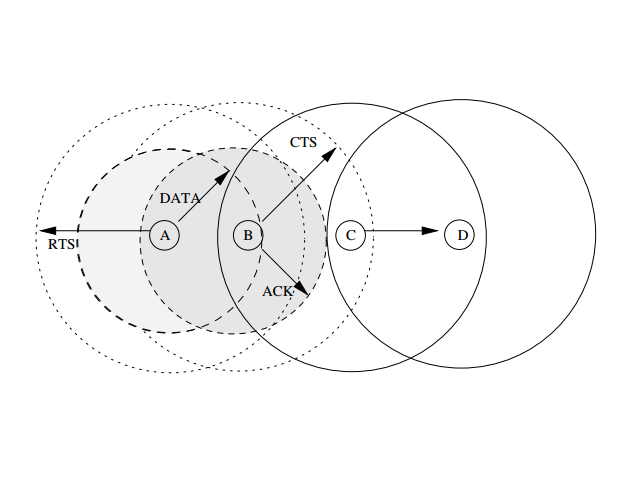
\epsfig{file=images/basic.png, width=8cm}
					\caption{Pursley et al. Power Control Scheme}
					\label{fig:basic_tpc}
				\end{figure}				
				A further extension of this work is presented in \cite{jung2002power}, since the power control scheme shown in \cite{pursley2000energy} may potentially decrease the throughput and increase energy consumption in some scenarios. The main root cause are the collisions may occur due to the Hidden-Node problem, since neither CTS nor RTS frames may not be listened by some interfering nodes. Therefore, the new proposed scheme, which is named Power Control MAC (PCM), deals with the aforementioned kind of asynchronies by forcing nodes to transmit periodically DATA at the maximum power. Figure \ref{fig:pcm} shows the power used during a DATA/ACK transmission if using PCM, which is set to $p_{max}$ during $20 \mu s$ every $190 \mu s$. These values are predefined because the EIFS value specified by the DCF when data rate is 2 Mbps is equal to $212 \mu s$. Thus, power level during DATA transmission is increased once at each EIFS interval to the time at which it is minimum.
				\begin{figure}[h!]
					\centering
					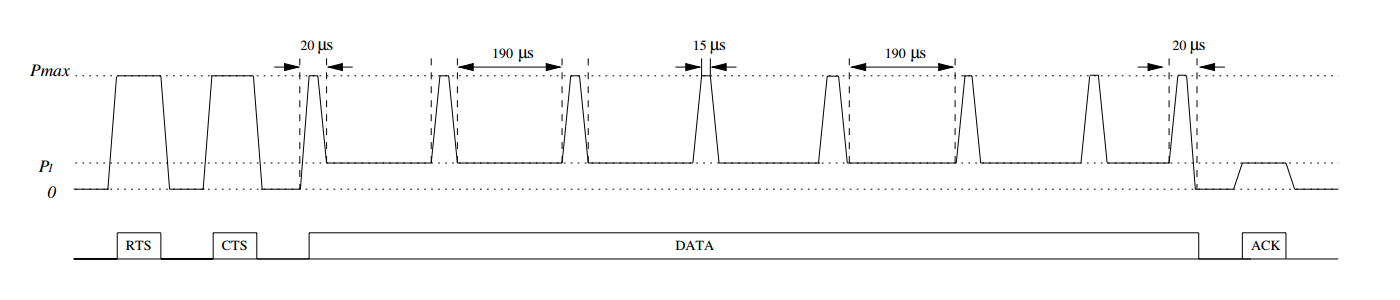
\epsfig{file=images/pcm.png, width=13cm}
					\caption{PCM Scheme}
					\label{fig:pcm}
				\end{figure}
				This power control scheme is validated in several network topologies, so that remarkable improvements are shown at saving energy. In particular, savings of about 10\% are achieved whilst obtaining very similar throughput values with respect to current IEEE 802.11 operation. Despite the main goal of the PCM scheme used is to reduce energy consumption, it implicitly allows improving the spatial reuse, which shows that using the necessary power during a wireless transmission can be beneficial for the network capacity. 
				
				Similarly to previous reviewed approaches by using RTS/CTS frames, the authors in \cite{lei2015performance} attempt to improve the throughput of OBSSs by using an RTS/CTS modification that incorporates different Network Allocation Vector (NAV) timers. Thus, despite RTS and CTS packets are transmitted at the maximum power, a higher number of parallel transmissions can be carried out, since the new NAV timers only captures the RTS/CTS operation. However, this solutions appears to be quite rigid and to behave properly only at few situations.
				
				Another important research line for TPC is based on measuring and/or inferring the channel characteristics. The authors in \cite{chaves2014adaptive} show the benefits of tuning the transmit power in terms of interference, and without affecting to the MCS granted by the Channel State Information (CSI) from previous transmissions. In \cite{oteri2013advanced}, the authors also study the potential of TPC. In particular, four TPC schemes are provided for theoretical comparison:
				\begin{itemize}
					\item No TPC: devices transmit at the maximum transmit power.
					\item Basic TPC: devices transmit at the minimum necessary power to reach the farthest device in their network.
					\item Unfiltered TPC: the power is adjusted to the minimum necessary per link communication, but beacons to the minimum required power for reaching the farthest device.
					\item Filtered TPC: an IIR filter is used to adjust the transmit power $y(n)$, which is computed as $y(n) = a \cdot y(n-1) + (1-a) \cdot x(n)$, where  $y(n-1)$ is the previous estimated transmit power, and $x(n)$ is the instantaneous power needed.
				\end{itemize}  
				Several experiments are done regarding the uplink and the downlink performance for several combinations of the introduced approaches, showing the potential of providing such kind of power control mechanism. In addition, it also introduces the concept of Fractional-CSMA/CA, which aims to coordinate the transmissions within different BSSs in order to make the most of TPC. Thus, the number of parallel transmissions can be increased without suffering collisions by hidden node (refer to Figure \ref{fig:fcsma}). The concept of F-CSMA/CA is also interesting to even improve the TPC operation, since it would allow to make a step further for enhancing spatial reuse. However, it requires a strong coordination that appears to be infeasible in the uncoordinated scenarios of interest for this work.
				\begin{figure}[t!]
					\centering
					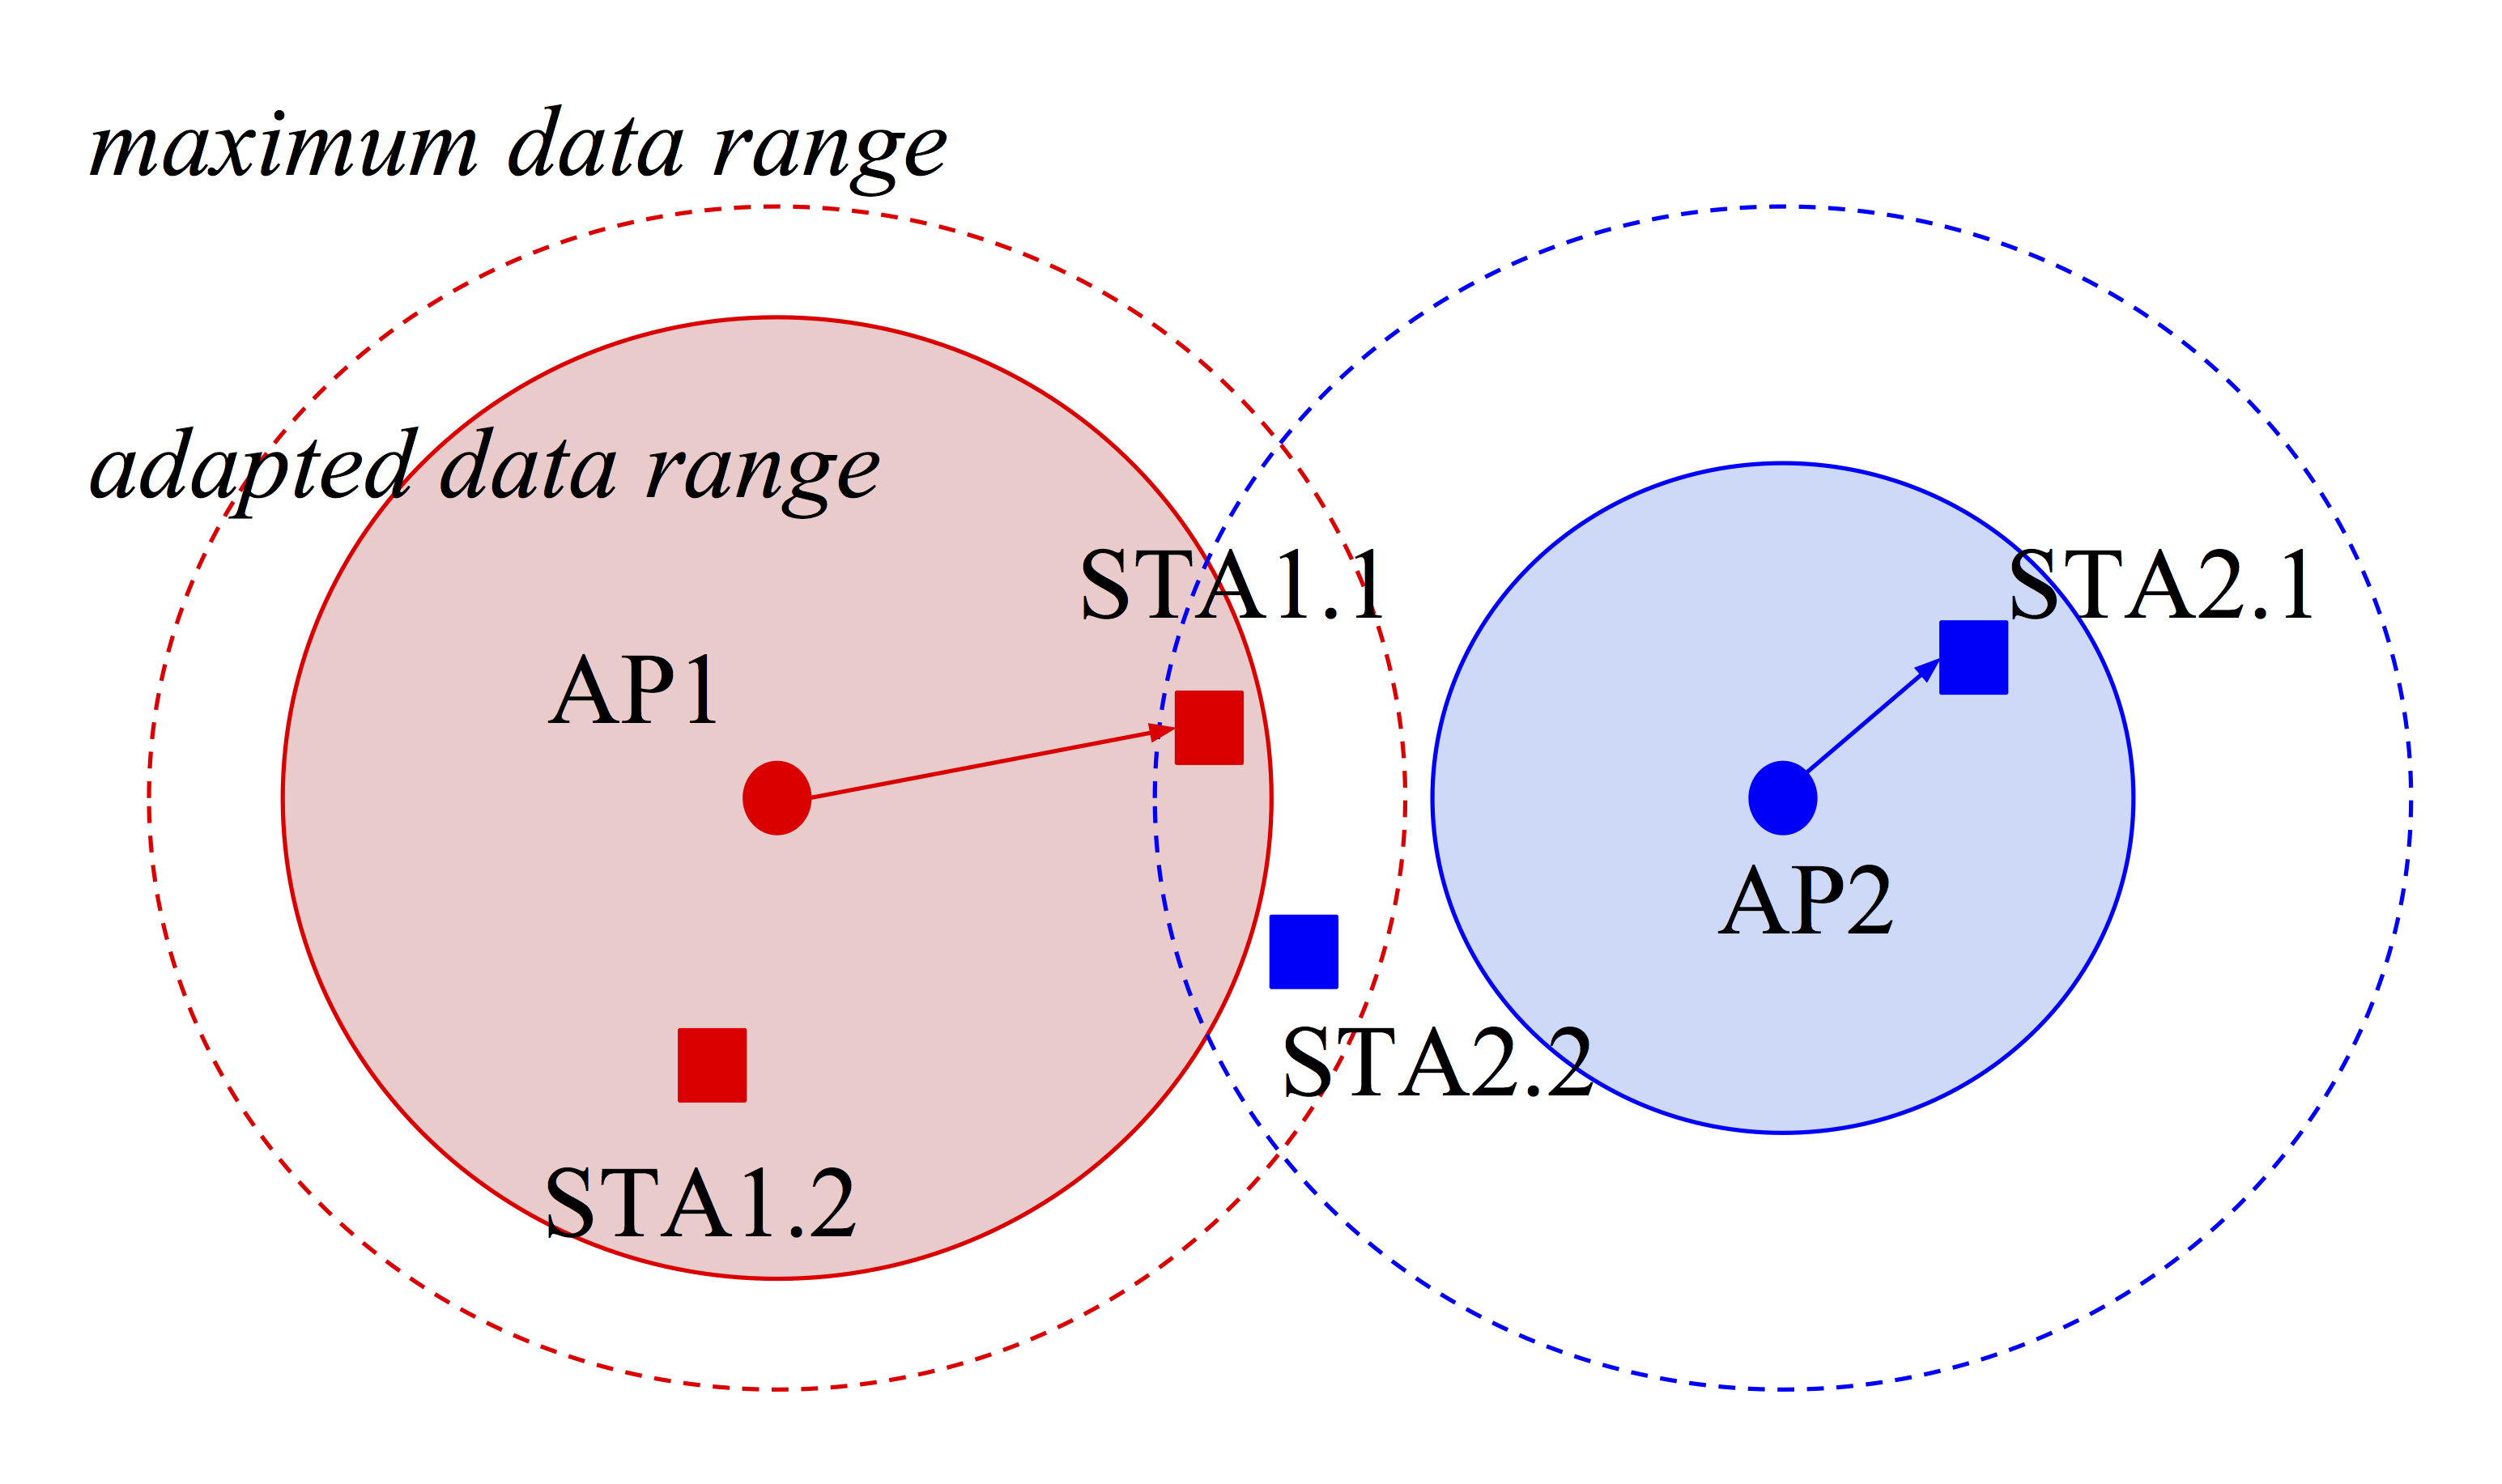
\epsfig{file=images/fcsma.png, width=11cm}
					\caption{F-CMSA operation. The orange AP uses a higher transmit power to reach its farthest STA. At the same time, the blue AP transmits to a close device, so that transmit power does not affect the other ongoing transmission. This scheduling is provided by a central entity. }
					\label{fig:fcsma}
				\end{figure}	
			
				Another approach that uses observations to determine the power level to be used is shown in \cite{gandarillas2014dynamic}. In it, the authors propose a decentralised system called ``DTPC", which is based on triggered thresholds. Transmission power, channel occupancy and link status are the main inputs of the algorithm for modifying the transmit power. Two simulations are carried out to validate the DTCP algorithm. The first one only considers are very simple scenario in which interferences from two APs are shown to be minimised through DTPC. The second one analyses the impact of applying DTPC in two nodes, showing improvements in both energy consumption and throughput. In both cases, adjacent channels are used. The main problem is that thresholds are set empirically (based on simulations), so it may be dangerous to apply this to other scenarios different than from simulations.	Moreover, a centralised TPC mechanism is proposed in \cite{tang2014joint}. It also includes and Rate Adaptation (RA), since the current Auto-Rate Fall back (ARF) mechanisms only consider channel fading. An interesting contribution of this work is the creation of subgroups of WLANs, according to their neighbouring relationship in terms of interference. This allows defining independent power differences between devices in the same group. This power difference is useful to avoid asymmetric links. The main drawback of this work is that graphs can become very large, and that using the channel as a decision parameter is not strong enough to determine a relationship between two nodes. As a result, many nodes in the same group may lack of mutual interference. Similarly, the authors in \cite{elbatt2000power} aim to solve the energy saving problem in ad-hoc WNs by using a protocol that dynamically adjusts the power level, so that throughput is maximised. The core idea is to create clusters, so that transmit power can be adjusted accordingly. Then, a minimum power routing scheme is provided to find the shortest path in terms of power consumption
				
				Finally, we find a different TPC approach that is also worth to mention (\cite{ebert2000energy}), since their authors show a strong relationship between the transmit power and the packets size in order to enhance energy consumption is WLANs. In particular, they adjust the transmit power according to the packet size, based on prior experiments. Furthermore, they show that the energy used to transmit one payload bit in a long run is given by:
				\begin{equation}
				E_{bit_res} = \frac{\sum_{i=1}^N P_{tx,i} \cdot B_{all,i}}{B_{succ}} \cdot T_{bit},
				\nonumber
				\end{equation}
				where N is the number of power levels, $P_{tx,i}$ is the transmit power level $i$, $B_{all,i}$ is the packet size (including headers), $B_{succ}$ is the number of successfully received bits, and $T_{bit}$ is a bit time. 
				
				By now, we have referred to the relationship between the throughput enhancement and the power consumption reduction, which is granted by TPC. However, this situation is likely to occur in dense environments at which the interference limits the network performance. Notwithstanding, improving the network throughput through TPC does not necessarily imply an energy saving, but the opposite. For instance, a high transmit power would be required to enhance the performance of an isolated network in which the AP is far enough from a STA. The energy consumption issue is almost approached in the context of wireless ad-hoc networks, due to the trade-off them present. On the first hand, increasing the power level increases the transmission range, but it may generate interferences that lead into collisions or starvation. On the other hand, using a low power level allows reducing the interference, but a higher number of hops may be required for a packet transmission. As a final remark, we emphasise the importance of providing a solution that properly works in case of coexisting with legacy devices. In \cite{broustis2010measurement}, it is argued that using TPC in such environments can be detrimental to the aggregate performance. 
				
				Table \ref{tbl:tpc} summarises the most important reviewed works on transmit power adaptation in wireless networks.
				\begin{table}[t!]
					\centering
					\resizebox{\textwidth}{!}{\begin{tabular}{|c|l|c|l|l|}
							\hline
							\multicolumn{1}{|c|}{\textbf{Work}} & \multicolumn{1}{c|}{\textbf{Presented Approach}} & \textbf{\begin{tabular}[c]{@{}c@{}}Centralised/\\ Decentralised\end{tabular}} & \multicolumn{1}{c|}{\textbf{Positive Aspects}} & \multicolumn{1}{c|}{\textbf{Negative Aspects}} \\ \hline
							\cite{oteri2013advanced} & \begin{tabular}[c]{@{}l@{}}Minimises transmit power while \\ preserving the maximal rate to\\ minimise interference\end{tabular} &  Both & \begin{tabular}[c]{@{}l@{}}  Decentralised approach: \\$\bullet$ Introduces IIR filters to  \\ adjust TPC \\Centralised approach:  \\$\bullet$ Introduces the interesting  \\concept of F-CSMA \end{tabular} & \begin{tabular}[c]{@{}l@{}}Decentralised approach:\\$\bullet$ Depends on rate adaptation \\ $\bullet$ Only applies to dense scenarios\\ $\bullet$ May generate asymmetric links \\ $\bullet$ Heuristic parameters assignment \\is done \\ Centralised approach: \\$\bullet$ Infeasible in uncoordinated scenarios\\\end{tabular} \\ \hline
							\cite{lei2015performance} & \begin{tabular}[c]{@{}l@{}}Presents a modification of\\ RTS/CTS that introduces\\ several NAV timers, so that\\ adjusting transmit power \\ does not increase the number \\of collisions\end{tabular} & Decentralised & \begin{tabular}[c]{@{}l@{}}$\bullet$  Provides fairness \\ $\bullet$ Improves the network \\ throughput \end{tabular} & \begin{tabular}[c]{@{}l@{}}$\bullet$ Only useful at few specific cases.\\ $\bullet$ Lack of evidences in realistic scenarios.\end{tabular} \\ \hline
							\cite{gandarillas2014dynamic} & \begin{tabular}[c]{@{}l@{}}A real-time mechanism based \\on triggered thresholds is \\provided to modify the \\  transmit power according\\ to the link status and the \\ channel occupancy\end{tabular} & \multicolumn{1}{l|}{Decentralised} & \begin{tabular}[c]{@{}l@{}}$\bullet$  No extra signalling is \\ required \end{tabular} & \begin{tabular}[c]{@{}l@{}} $\bullet$ Thresholds are set empirically\\ $\bullet$ Lacks of applicability in real scenarios\end{tabular} \\ \hline
							\cite{tang2014joint} & \begin{tabular}[c]{@{}l@{}}Adjusts transmit power together \\ with the data rate\end{tabular} & Centralised & \begin{tabular}[c]{@{}l@{}}$\bullet$ A clustering approach is \\provided in order to avoid \\ link asynchronies\end{tabular} & \begin{tabular}[c]{@{}l@{}}$\bullet$ The clustering algorithm can lead to \\ inefficient and large graphs, specially\\ in dense environments\\ $\bullet$ The cost of centralisation is not studied\\ $\bullet$ Coexistence with legacy devices is not\\ considered\end{tabular} \\ \hline						
					\end{tabular}}
					\caption{State-of-the-Art on Transmission Power Control}
					\label{tbl:tpc}
				\end{table}										
							
		%%%%%%%%%%%%%%%%%%%%%%%%%%%%%%%%%%%%%%%
		% SoA CST										         %%%%%%%%%%%%%
		%%%%%%%%%%%%%%%%%%%%%%%%%%%%%%%%%%%%%%%						
		\section{Carrier Sense Threshold Adjustment}
		\label{section:cca}
			In addition to proper frequency allocation and power control mechanisms, the Carrier Sense Threshold (CST) adjustment is key to improve the spatial reuse. By tuning the sensitivity at the receiver, it is possible to increase the number of parallel transmissions, thus maximising the aggregate throughput. In \cite{jamil2014improving}, the authors explore the possibilities to improve the capacity in IEEE 802.11 WLANs by modifying the CST. To do so, they present a typical OBSS deployment (Figure \ref{fig:jamil_2014_1}) and study its performance for different CCA thresholds. An interesting pattern is shown regarding the CST and aggregate throughput relationship (Figure \ref{fig:jamil_2014_2}). Moreover, the presence of legacy devices is shown to negatively affect to the overall performance.
			\begin{figure}[t!]
				\centering
				\begin{subfigure}[b]{0.4\textwidth}
					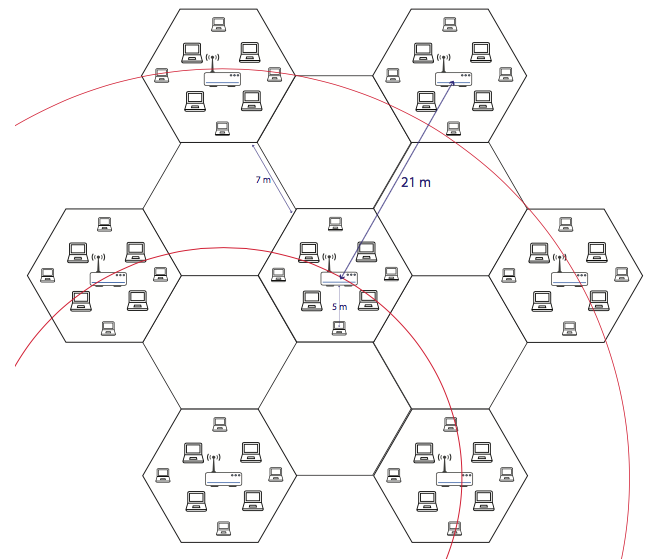
\includegraphics[width=\textwidth]{images/jamil2014_1}
					\caption{Network topology}
					\label{fig:jamil_2014_1}
				\end{subfigure}
				\begin{subfigure}[b]{0.4\textwidth}
					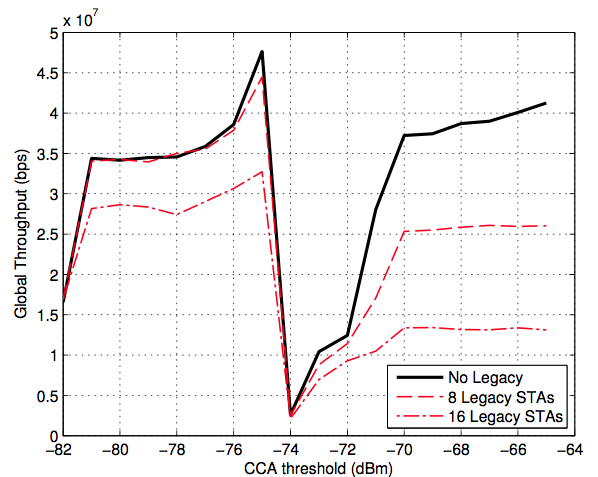
\includegraphics[width=\textwidth]{images/jamil2014_2}
					\caption{Aggregate throughput for different CST levels}
					\label{fig:jamil_2014_2}
				\end{subfigure}		
				\caption{IEEE 802.11ax Residential scenario}
				\label{fig:jamil_2014}
			\end{figure}		
		
			As for TPC, the TGax also introduces several limitations for adjusting the CST \cite{tgax2016draft}, so that the minimum and maximum allowed sensitivity levels ($\text{OBSS\_PD}_{min}$ and $\text{OBSS\_PD}_{max}$) are determined to be -82 dBm and -62 dBm, respectively. With that, a STA can dynamically select a sensitivity level ($\text{OBSS\_PD}_{level}$) during its operation under SR mode, which is bounded by the aforementioned minimum and maximum levels:			
			\begin{equation}
				\resizebox{1\hsize}{!}{$\text{OBSS\_PD}_{level} \leq max\Big(\text{OBSS\_PD}_{min}, min\big(\text{OBSS\_PD}_{max}, \text{OBSS\_PD}_{min} + (\text{TX\_PWR}_{ref}-\text{TX\_PWR})\big)\Big),$
				\nonumber}				
			\end{equation}
			where $\text{TX\_PWR}$ is the STA's transmission power in dBm at the antenna connector, and $\text{TX\_PWR}_{ref}$ is set to 21 or 25 dBm according to the device capabilities\footnote{$\text{TX\_PWR}_{ref} = 21 dBm$ for non-AP STAs and for an AP with the Highest NSS Supported M1 subfield in the Tx Rx HE MCS Support field of its HE Capabilities element field equal to or less than 1. $\text{TX\_PWR}_{ref} = 25 dBm$ for an AP with the Highest NSS Supported M1 subfield in the Tx Rx HE MCS Support field of its HE Capabilities element field equal to or greater than 2.}.
			The obtained $\text{OBSS\_PD}_{level}$ varies for each channel width used, as shown in Table \ref{tbl:sensitivity_channel_width}.
			\begin{table}[h!]
				\centering
				\begin{tabular}{|c|l|}
					\hline
					\textbf{Channel width} & \multicolumn{1}{c|}{\textbf{$\text{OBSS\_PD}_{level}$}} \\ \hline
					40 MHz                 & $\text{OBSS\_PD}_{level}$ + 3 dB                        \\ \hline
					80 MHz                 & $\text{OBSS\_PD}_{level}$ + 6 dB                        \\ \hline
					160 MHz or 80+80 MHz   & $\text{OBSS\_PD}_{level}$ + 9 dB                        \\ \hline
				\end{tabular}
				\caption{IEEE 802.11ax specification for the sensitivity per channel width}
				\label{tbl:sensitivity_channel_width}
			\end{table}			
		
			The most important approach seen so far for adjusting the CST in IEEE 802.11 WLANs is the Dynamic Sensitivity Control (DSC) algorithm, which has been proposed by the TGax \cite{smith2015dynamic}. The DSC algorithm aims to distributively find an appropriate level of CST in each non-AP station of a WLAN, with the aim of maximizing the number of parallel transmissions and the aggregate throughput. DSC periodically adjusts the CST of a wireless device given the information retrieved from Received Signal Strength Indicator (RSSI) measurements. The operation mode of DSC is graphically represented in Figure \ref{fig:dsc_flowchart}.				
			\begin{figure}[t!]
				\centering
				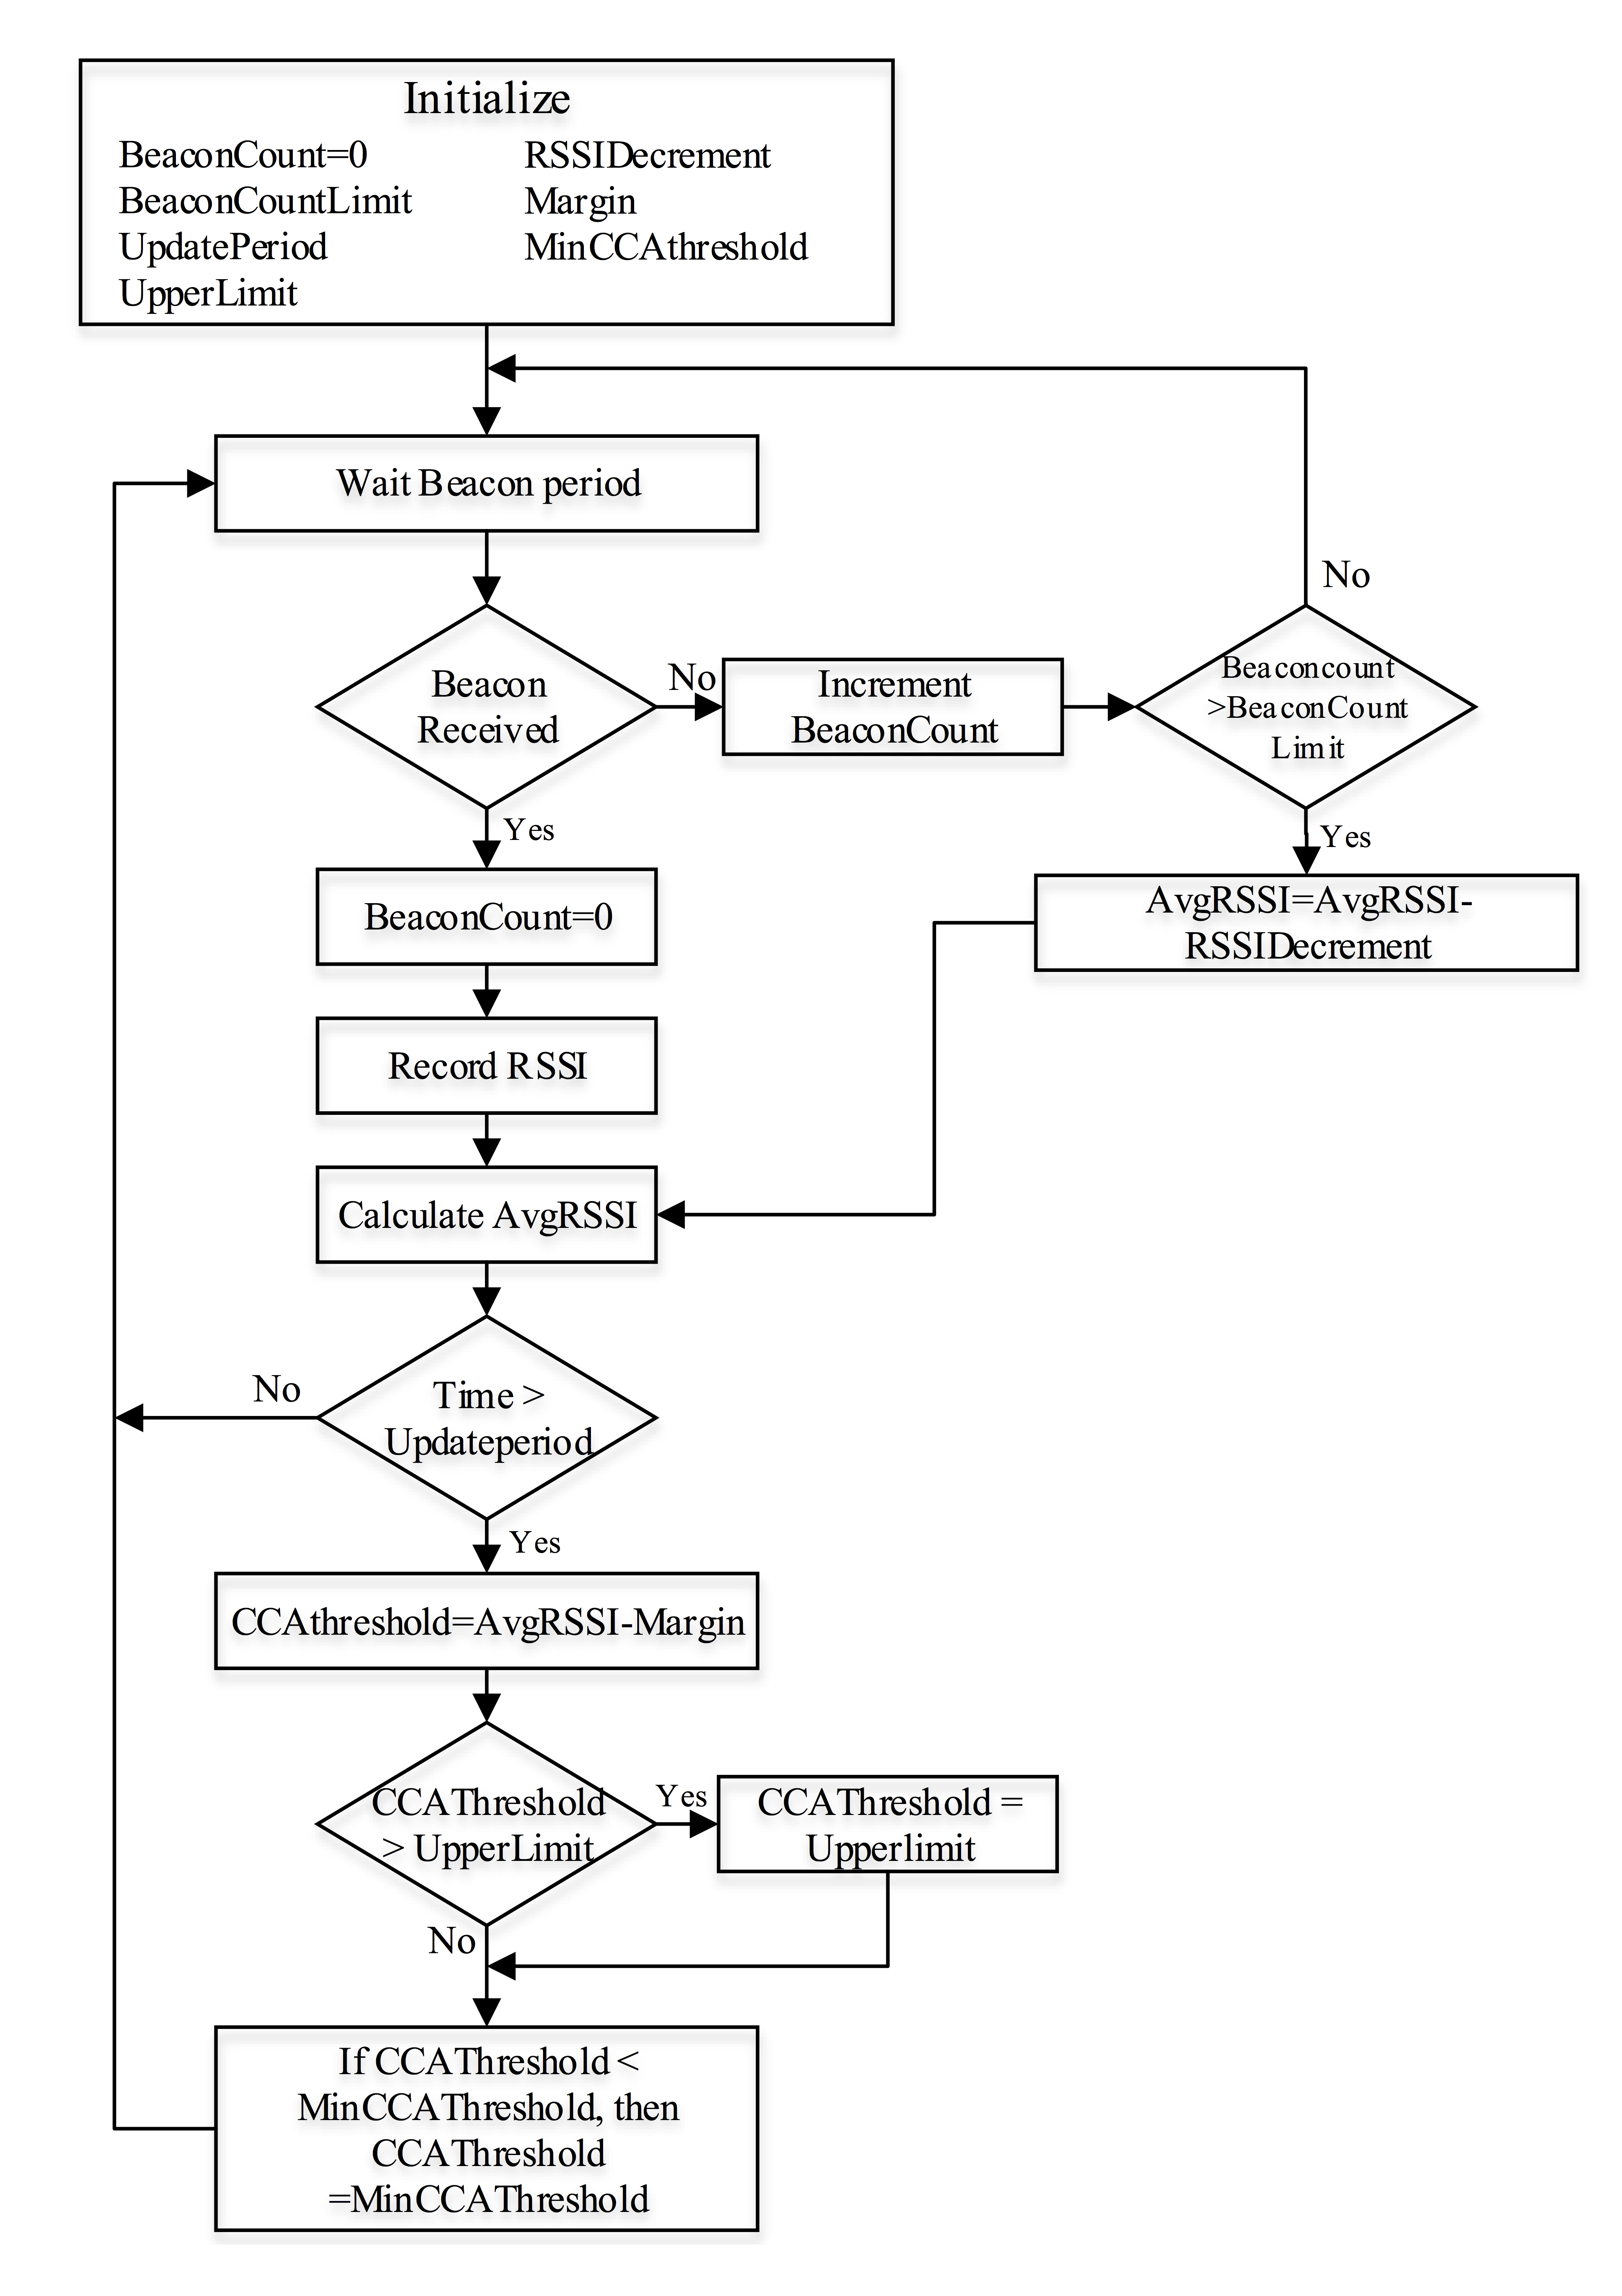
\epsfig{file=images/DSC.png, width=9cm}
				\caption{Dynamic Sensitivity Control operational mode}
				\label{fig:dsc_flowchart}
			\end{figure}
		
			In particular, a station accumulates the Received Signal Strength Indication (RSSI) of  each  sensed  beacon until the \textit{UpdatePeriod} is reached. An average of the RSSI (\textit{AvgRSSI}) is maintained for adjusting the CST later. In parallel, it is counted the number of beacons missed during an \textit{UpdatePeriod}. At each Beacon Interval (BI) it is compared the number of lost beacons (\textit{BeaconCount}) with a maximum threshold (\textit{BeaconCountLimit}). In case \textit{BeaconCount} is greater than \textit{BeaconCountLimit}, the average RSSI is decreased by a default value (\textit{RSSIDecrement}) with the aim of decreasing the CST and thus listen further away to receive more beacons. Finally, after the \textit{UpdatePeriod} is reached, it is computed the new CST value between a minimum and a maximum boundaries (\textit{LowerLimit} and \textit{UpperLimit}, respectively). The CST is computed as \textit{AvgRSSI} minus a margin, which is a positive number (typically from 5 to 25).
					
			An evaluation of the DSC algorithm is provided in \cite{afaqui2015evaluation}, which 
			applies to non-AP stations in the residential scenario introduced by the TGax. On the one hand, it is shown that the overall throughput can be increased up to a 20\% with respect to legacy networks if using DSC. On the other hand, the application of DSC at uncoordinated WNs may generate a significant increase in the number of hidden nodes, which can potentially harm the overall throughput due to collisions. In fact, the increase in hidden nodes is measured to be the 60\% in the best of the cases, and the 160\% in the worst situation. Best results are obtained by using smart channel selection and fixed modulation coding scheme, while the worst results are obtained by using randomising both parameters. With that, we see that DSC allows enhancing the overall throughput by allowing a higher number of parallel transmission without adding signalling. However, it potentially increases the number of hidden-nodes within an overlapping WLAN, which may be counter productive if the effects of packet collisions result into a worse throughput performance.
			
			
						
	
						
			
			
			A further extension of DSC can be found in \cite{afaqui2016dynamic}, which intends to cover both UL and DL situations by also adjusting CST on the APs, as well as the initial DSC approach does not take into account that starvation in APs may occur during DL transmissions. Figure \ref{fig:enhanced_dsc} shows the flowchart of the process described above.The DSC-AP algorithm works as follow:
			\begin{itemize}
				\item The AP records the RSSI of the received frames (either data packets or ACKs) during a period called \textit{UpdatePeriod}. The collected frames come from both associated stations and neighboring APs.
				\item A moving maximum RSSI ($max\mathrm{RSSI}$) is maintained for the frames received from other APs, in order to know which is the most interfering coexistent WLAN.
				\item Similarly, a minimum RSSI ($min\mathrm{RSSI}$) is maintained for the frames received from the STAs within the WLAN, in order to detect the farthest STA (in fact, the STA from which the AP receives the poorest signal).
				\item When the \textit{UpdatePeriod} is reached, a new CST between specific boundaries (\textit{LowerLimit} and \textit{UpperLimit}) is computed:
				$\mathrm{CST}_{AP} = min(max(min\mathrm{RSSI},max\mathrm{RSSI})-Margin,min\mathrm{RSSI})$, where \textit{Margin} is a value between 18 and 25 dB for indoor scenarios (path-loss factor ($\alpha$) is 0.3). 
			\end{itemize}
			
			A set of simulations is used to show the benefits of using DSC-AP (in APs) in combination with DSC (in non-AP stations). Note that the scenario used is the same as for DSC evaluation seen in \cite{afaqui2015evaluation} (refer to Figure \ref{fig:TGax_scenario}). Among different settings (asymmetric traffic, ), we highlight the application of the algorithms together with optimal channel selection, so that an improvement of the 32\% in the overall throughput is achieved with respect to legacy IEEE 802.11 performance. In addition, fairness is increased up to 16\% because of the reduction of exposed nodes, which supposes noticing less starvation situations. The derived problems of using DSC-AP are also related to the increase of hidden nodes and collisions probability. But again, for the particular presented scenario, the obtained throughput is better despite the significant increase of the Frame Error Rate (FER).	
			\begin{figure}[h!]
				\centering
				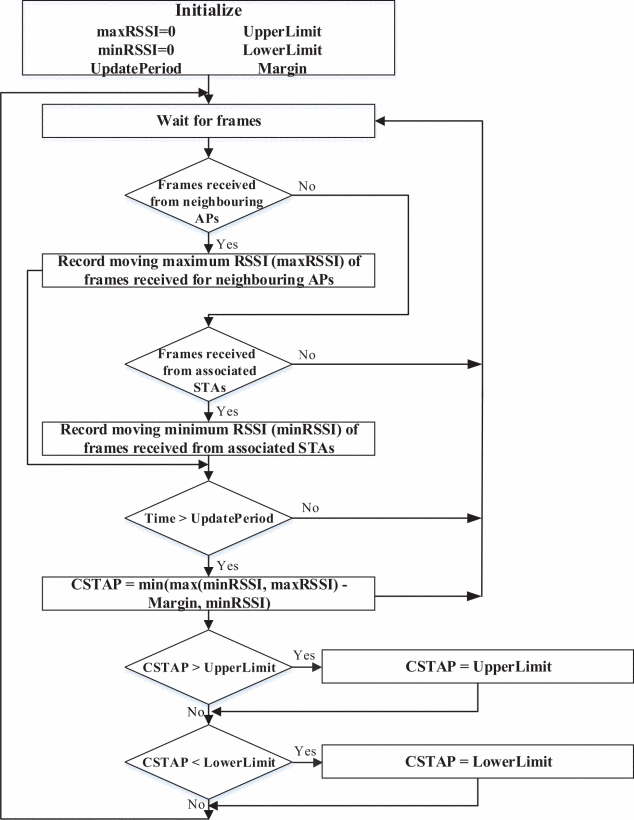
\epsfig{file=images/enhanced_DSC.png, width=9cm}
				\caption{DSC-AP flowchart}
				\label{fig:enhanced_dsc}
			\end{figure}
			
			Another contribution of Afaqui et al. on sensitivity adjustment is \cite{afaqui2016rtscts}, which consists in combining DSC with RTS/CTS activation in stations. In particular, three approaches for enabling RTS/CTS in a given station are shown in combination with DSC:	
			\begin{itemize}
				\item \textbf{Method 1:} a set of devices within a WLAN is decided to use RTS/CTS according to a given threshold of FER, which is based in the average FER of the network ($\mathrm{FER}_{Thresh} = \delta \times \mathrm{FER}_{avg}$). Then, an AP maintains the usage of RTS/CTS for each of its associated STA according to their FER information ($f_i$). In particular, RTS/CST is activated for a given STA $i$ if $f_i$ is equal or higher than the $\mathrm{FER}_{Thresh}$. Otherwise, RTS/CST is disabled. 
				Note that the AP of a given WLAN needs to know the FER information of its associated STAs, which implies adding communication overhead (also for activation/deactivation of RTS/CTS for each pair of nodes when required). In this case, the necessary information to carry out this operation is assumed to be known by the nodes in the network.
				\item \textbf{Method 2:} To avoid using the extra overhead for maintaining the $\mathrm{FER}_{avg}$, in this method the AP selects a fixed percentage $\eta$ of STAs and activates RTS/CTS in the ones that have higher FER. The way $\eta$ is chosen is not described, but this approach may lead to many problems because it can easily underestimate/overestimate the number of nodes that need to use RTS/CTS, which may lead to collisions and unnecessary overhead, respectively. 
				\item \textbf{Method 3:} In this case, all the APs use the number of hidden nodes noticed in all of their STAs to select a percentage $\gamma$ of nodes to use RTS/CTS (the ones with higher number of hidden nodes are selected). In this case, not only communication overhead is added, but extra computation in all the nodes to find hidden nodes (which probably cannot be done with complete accuracy).
			\end{itemize}
			
			Simulations done in this case contemplate the same scenario seen in Subsections \cite{afaqui2015evaluation} and \cite{afaqui2016dynamic}. As Method 1 with $\delta = 0.6$ is shown to perform better in terms of throughput improvement, it is used along all the simulations. Henceforth, the maximum improvement shown in the simulations is an increase of approximately 55\% in the overall throughput with respect to legacy IEEE 802.11 performance when using frames of size 2302 Bytes. In this setting, the FER is reduced almost 40\% and fairness is increased in 30\%. Using smaller frames (1000 and 1600 Bytes) it is shown a higher reduction of the FER, but a lower increase of the throughput (15\% and 25\%, respectively) and a decrease of the fairness (4\% and 9\%, respectively).	The fact of enabling RTS/CTS dynamically allows reducing the effects of hidden nodes in terms of collisions without adding too many overhead due to RTS/CTS transmissions, as well as it is only used in nodes that really require it. In opposite, many communication overhead is added to decide which nodes must use RTS/CTS, which has not been quantified for showing the resulting throughput when using this approach.
	
			
			\cite{afifi2016throughput} \textcolor{red}{TODO} In this paper, we provide a theoretical framework to evaluate the aforementioned tradeoff. We also propose a centralized fairness mechanism (CFM), in which STAs switch between an adaptive phase (CCA adaptation is allowed) and a fixed phase (legacy and HE STAs use the same CCA threshold). We formulate an optimization problem with the objective of determining the optimal switching strategy that maximizes the network throughput while maintaining a lower bound on per-STA throughput. Finally, we validate the proposed mechanism using simulations.		
			
			
			
			
			\textcolor{red}{TODO: review \cite{selinis2016evaluation, zhong2016promise, kulkarni2015taming} for DSC evaluation.}
	
	
	
			\textcolor{red}{TODO: Table 2: CST adjustment}
			\begin{table}[h!]
				\centering
				\begin{tabular}{|l|l|l|l|l|}
					\hline
					\textbf{Work} & \textbf{Main Purpose} & \textbf{Centralised / Decentralised} & \textbf{Benefits} & \textbf{Drawbacks} \\ \hline
					{[}1{]} &  &  &  &  \\ \hline
					{[}2{]} &  &  &  &  \\ \hline
					{[}3{]} &  &  &  &  \\ \hline
				\end{tabular}
				\caption{Carrier Sense Threshold Adjustment State-of-the-Art}
				\label{tbl:cca}
			\end{table}
		
		%%%%%%%%%%%%%%%%%%%%%%%%%%%%%%%%%%%%%%%
		% TPC & CCA RELATIONSHIP		            %%%%%%%%%%%%%
		%%%%%%%%%%%%%%%%%%%%%%%%%%%%%%%%%%%%%%%				
		\section{TPC and CCA Relationship}
		\label{section:tpc_cst_relationship}
		
		
			There is a direct relationship between the CST, the distance between overlapping nodes, and the transmit power used. This is attempted to be capture in \cite{zhu2004leveraging}, where CST at devices in a mesh WNs is computed as a function of the distance between nodes, and assuming that the same transmit power is used. In particular, different CST equations are provided for grid and line topologies, since the interference pattern varies. In this case, all the devices are considered to be placed symmetrically. Thus, an ideal situation is proposed for planned and interference-free deployments (e.g. a rural sensors deployment). However, this approach turns out to be unrealistic in chaotic wireless deployments.
			
			
			As seen in Sections \ref{section:power_control} and \ref{section:cca}, adjusting either the transmit power or the CST can help to improve spatial reuse, but presents a set of trade-offs. To even improve them usage, there is a research line that argues a relationship between the power transmitted and the sensitivity threshold, which is based on the naive principle ``to shout, you need to listen more carefully".
			
			\textcolor{red}{TODO: references that show a relationship between CST and TPC}			
			
			\cite{oteri2015improved}
			
			TODO:  \cite{jamil2014improving} \cite{zhu2004leveraging}
			
			A very simple mechanism to adjust both TPC and CCA is shown in \cite{jamil2015preserving}, in which fairness improvement is the main goal (although the overall throughput is also enhanced). The behaviour of the mechanism just attempts to modify TPC and CCA as follows:
			\begin{itemize}
				\item Each time a beacon is received in a STA, it is measured a parameter to adapt both CST and transmit power: $\Delta_x = Rx_p - M - PCS_{default}$, where $Rx_p$ is the power received (depends on the power transmit and the attenuation loss), $M$ is a margin (in this case it is set to 20 dB), and $PCS_{default}$ is the default minimum CST (for channels of width 20 MHz, $PCS_{default}$ is -82 dBm).
				\item The difference of CCA and TPC is computed from $\Delta_x$ and a given ratio:
				$$\Delta_{TPC} = ratio \times \Delta_x$$
				$$\Delta_{CCA} = \Delta_x - \Delta_{TPC}$$
				\item Finally, the TPC and the CCA are modified by increasing/decreasing the obtained adaptation values:
				$$TPC = TPC - \Delta_{TPC}$$
				$$CCA = CCA + \Delta_{CCA}$$
			\end{itemize}	
			A representation of the algorithm is shown in the following image:	
			\begin{figure}[h!]
				\centering
				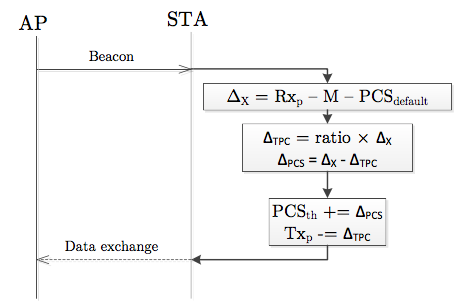
\epsfig{file=images/cca_tpc_adaptation_simple.png, width=7cm}
				\caption{Jamil et al. CCA and TPC adaptation algorithm}
				\label{fig:jamil_et_at_algorithm}
			\end{figure}
			
			The $ratio$ determines how much is adapted CCA and/or TPC, as setting it to 0 means only CCA adaptation, while setting it to 1 adjusts only the TPC. To adapt both CCA and TPC, so-called Balanced TPC and PCS Adaptation (BTPA), the chosen $ratio$ is 0.5, but during the simulations it is also shown the results of adapting CCA and TPC separately. The scenario consists in a cellular network composed by 7 APs that transmit data to 8 STAs each one.	The results are quite interesting, as the average throughput is increased by a 4 factor while preserving the fairness coefficient to 1:	
			\begin{figure}[t!]
				\centering
				\begin{subfigure}[b]{0.3\textwidth}
					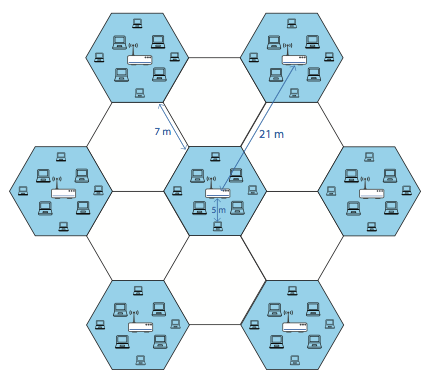
\includegraphics[width=\textwidth]{images/scenario_tpc_cca_adaptation_cellular}
					\caption{Simulation Scenario}
					\label{fig:jamil_et_al_scenario}
				\end{subfigure}
				\begin{subfigure}[b]{0.3\textwidth}
					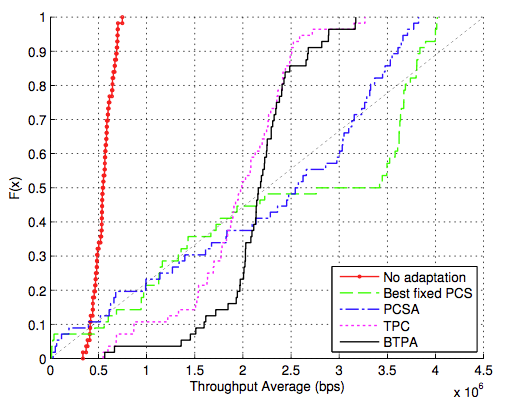
\includegraphics[width=\textwidth]{images/results_tpc_cca_adaptation_simple}
					\caption{Results}
					\label{fig:jamil_et_al_results}
				\end{subfigure}		
				\caption{Jamil et al. simulation scenario and results of CCA and TPC adaptation mechanism}
				\label{fig:jamil_et_al_scenario_and_results}
			\end{figure}	
			
			Despite being very simple, this mechanism allows improving the spatial reuse while preserving fairness. It would be interesting to test this proposal into denser and more chaotic scenarios, such as residential Wi-Fi deployments, to properly test its effectiveness and performance bounds.		
	
			\subsection{Tuning TPC, CCA and Data Rate in Multi-hop Wireless Networks}
			In \cite{kim2006improving} we also see the desire of finding a relation between the power transmitted and the CST, but it this case it is also considered the trade-off between the increase of the spatial reuse and the decrease of the data rate (directly related with the power transmitted). Thus, the aim of that work is to find a power/carrier sense threshold in which the network capacity is maximized, and the relation between the transmit power and the CST. Therefore, it is presented a decentralized algorithm that adjusts power and rate control at a node given its interference level it perceives. The goal is also to keep the highest possible data rate, while keeping minimal the generated interference towards neighbouring WLANs. To do so, first it is required to determine the minimum power to be used so that the receiver can properly decode the message, which is given by the following equation:
			\begin{equation}
			P^{min} \geq \frac{SINR_{r[1]}^{th}}{SINR} \cdot P^{max},
			\end{equation}
			where $SINR_{r[i]}^{th}$ is the required SINR at the received to sustain rate $r[i]$. The data rate depends of the SINR, and its values are defined at the table below:	
			\begin{figure}[h!]
				\centering
				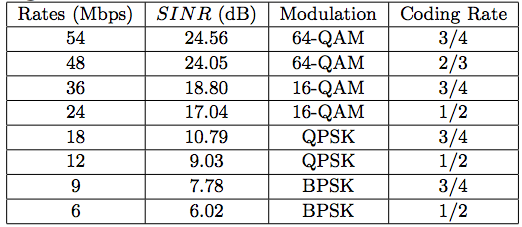
\epsfig{file=images/data_rate_table.png, width=8cm}
				\caption{Relation between SINR and data rate}
				\label{fig:data_rate_table}
			\end{figure}	
			Once the power transmitted is set, the CST should be set as the minimum value at which the incoming signal is sensed, which depends on the perceived interference:
			\begin{equation}
			I_{RX} \leq \frac{P^{min}_{tx}}{R^{\theta}_{max} \cdot SINR_{r[1]}^{th}},
			\end{equation}
			where $R^{\theta}_{max}$ is the maximum distance at which power $P^{min}_{tx}$ is sensed. The main problem is that the transmitter does not know the interference level $I_{RX}$ at the receiver. To deal this, the authors propose to set the CST at the transmitter as:
			\begin{equation}
			T_{CS}=\frac{P^{min}}{R^{\theta}_{max} \cdot \bigg( 1+(SINR_{r[1]}^{th})^{\frac{1}{\theta}} \bigg)^\theta},
			\end{equation}
			With that, it is ensured that the interference at the receiver will be at most $\frac{P^{min}_{tx}}{R^{\theta}_{max} \cdot SINR_{r[1]}^{th}}$, and that the minimal data rate will be sustained. Finally, to increase the power transmitted, it is presented an algorithm (\textit{Power and Rate Control, PRC}), which relies on finding the maximum SINR level to be achieved with a given tx power: if $SINR_{r[i]}^{th \geq SINR^{max}_{RX}}$ then data rate $r[i]$ is used. In particular the PRC starts when a node attempts to start a transmission. At that moment, the interference is monitored until it goes below the CST (channel is clear), which implementation details are shown in the image below:	
			\begin{figure}[h!]
				\centering
				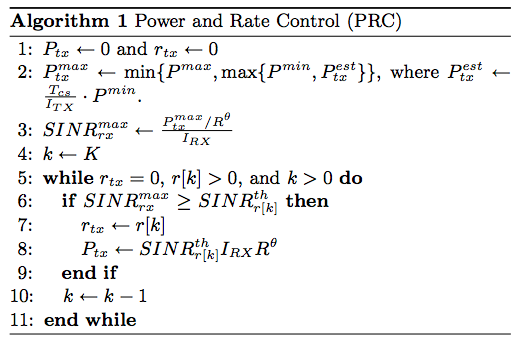
\epsfig{file=images/algorithm1.png, width=8cm}
				\caption{Relation between SINR and data rate}
				\label{fig:data_rate_table}
			\end{figure}	
			Then, the transmit power and the data rate are determined by the PRC algorithm:	
			\begin{figure}[h!]
				\centering
				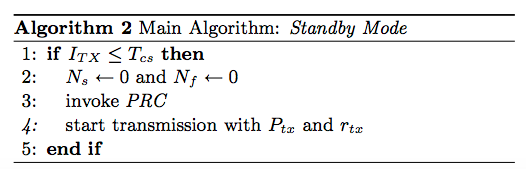
\epsfig{file=images/algorithm2.png, width=8cm}
				\caption{Relation between SINR and data rate}
				\label{fig:data_rate_table}
			\end{figure}	
			As other transmissions may start during the current ongoing transmission, the power transmit and the data rate must be adjusted dynamically as shown in the image below:	
			\begin{figure}[h!]
				\centering
				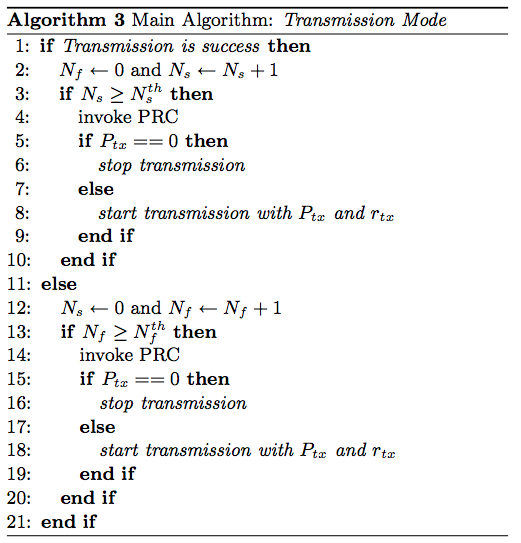
\epsfig{file=images/algorithm3.png, width=8cm}
				\caption{Relation between SINR and data rate}
				\label{fig:data_rate_table}
			\end{figure}	
			To monitor the variation of the interference level it is used the consecutive successful ($N^{th}_s$) and failed ($N^{th}_f$) transmissions. The demonstration of the algorithm's performance is shown through a set of simulations in ns-2 for different nodes densities (3, 10, 20, 30 and 50 transmitter-receiver pairs in a 300m $\times$ 300m area). The results show a significant increase with respect to the static setting on the aggregate throughput (up to 22\%) and the average saved power (up to 50\%).
			
			\subsection{Gibbs Sampler for Power Control}
			\label{section:gibbs_sampler_power_control}		
			It is well-known that modifying the TPC may result into asymmetries in the coexistence networks that may generate starvation in a higher probability than if using always the same configuration \cite{kawadia2005principles}. In consequence, in \cite{mhatre2007interference} it is defended that tuning TPC and CCA is a must if the goal is to improve spatial reuse in WLANs. For that, it is 
			shown how network links in a coexistence situation can remain symmetric if the power transmitted and the sensitivity threshold are adjusted together. Considering that the sensitivity $C_i$ of a given node for a given transmission must be $C_i =(\alpha_i + 1)N_0$, where $N_0$ is the floor noise level and $\alpha_i >>1$ is a variable that takes into account the shadow fading variations\footnote{In the 2.4 and 5.2 GHz frequency range, there variations are on the order of 10-14 dB [10]}, the relationship between the power transmitted $P_i$ and $\alpha_i$ prevents to generate starvation only if links are considered to be symmetric:
			\begin{equation}
			N_0 + P_j d_{i,j} \geq C_i \rightarrow \frac{d_{i,j}}{N_0} \geq \frac{\alpha_i}{P_j} \iff 
			N_0 + P_i d_{i,j} \geq C_j \rightarrow \frac{d_{i,j}}{N_0} \geq \frac{\alpha_j}{P_i}
			\end{equation}	
			The above inequalities show that a higher power entails sensitivity to be lower (\textit{if you want to shout, you need to listen more carefully}). Then, it is shown the objective function to determine the optimum settings (with respect to network capacity) for the constant C. As the goal is to minimize the sum of the potential delays of all users in the network (which is the inverse of long term throughput [8]), the objective function is:
			\begin{equation}
			\mathcal{F}(\boldsymbol{P,C})=\sum_{\text{All APs } i}  \bigg[ \sum_{\text{client } u \in \text{cell } i} \frac{1}{r_u(i)} \bigg],
			\end{equation}
			where $r_u(i)$ is the rate experienced by node $u$ in WLAN $i$, which depends on the experienced SINR. The previous function is approximated to:	
			\begin{equation}
			\mathcal{F}(\boldsymbol{\alpha},\mathcal{C})\equiv \sum_{i}  \text{U}_i^2 \cdot D_i(\alpha_i, \mathcal{C}) \cdot \bigg( 1 + \sum_{j\neq i}  1_{\Big\{ \frac{c_{d_{ji}}}{\alpha_j}  \geq \alpha_i N_0 \Big\}} \bigg) = \mathcal{E}(\boldsymbol{\alpha},\mathcal{C}),
			\end{equation}
			where $\text{U}_i$ is the number of clients in cell $i$, and $D_i(\alpha_i, \mathcal{C})$ is the average delay experienced by nodes in WLAN $i$. The second part of the equation represents the share of the channel with other WLANs and, thus the transmissions opportunities. So, the goal is to minimize $\mathcal{E}(\boldsymbol{\alpha},\mathcal{C})$ by tuning $\alpha$ and $\mathcal{C}$, representing the power transmitted and the sensitivity, which is done in a distributed manner through the Gibbs sampler. The algorithm implementation does the following steps after the timer of AP $i$ expires at time $t$ (the timer is an exponentially distributed variable with average $t_a$):
			\begin{itemize}
				\item Compute the temperature parameter as $T=\frac{K}{log_2(2+t)}$
				\item For each possible state $x \in Q_i$, compute the local energy as 
				$$\mathcal{E}(x,Z_i) = \text{U}_i^2 \cdot D_i(x) + \sum_{j:j\neq i} \Big\{ \text{U}_i^2 \cdot D_i(x) + \text{U}_j^2 \cdot D_j(X_j)\Big\} 1_{\Big\{ c_{ji}  \geq X_j + x \Big\} }$$
				\item Compute the corresponding state probability
				$$\pi(x) = \frac{e^{-\frac{\epsilon_i(x,Z_i)}{T}}}{\sum_{l:y\in Q_i} e^{-\frac{\epsilon_i(y,Z_i)}{T}}}$$	
				\item Sample a random variable according to $\pi(.)$ and select the resulting state
			\end{itemize}
			
			Finally, the power control algorithm is tested with OPNET simulator by focusing on 8 APs and 26 clients from a total of 72 APs and 288 clients (4 per AP). The reason of placing so much devices and then sub-sampling them is for randomly represent a plausible scenario and to take a representative proportion of it. For the Gibbs sampler time-ticks it is used the beacon intervals (100 ms), so that it is shown that the algorithm converges within 300 BI ($=30 s$). With that, it is shown how the average throughput is increased by a $290\%$. The interesting thing is that the initial premise is hold, since the power transmitted per AP is inversely proportional to the sensitivity.
			
			\begin{figure}[h!]
				\centering
				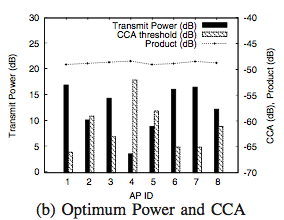
\epsfig{file=images/gibbs_results.png, width=8cm}
				\caption{Power transmitted and sensitivity per AP after applying Gibbs sampler}
				\label{fig:gibbs_results}
			\end{figure}
		
			\textcolor{red}{TODO: Table 3: all together}
			\begin{table}[h!]
				\centering
				\begin{tabular}{|l|l|l|l|l|}
					\hline
					\textbf{Work} & \textbf{Main Purpose} & \textbf{Centralised / Decentralised} & \textbf{Benefits} & \textbf{Drawbacks} \\ \hline
					{[}1{]} &  &  &  &  \\ \hline
					{[}2{]} &  &  &  &  \\ \hline
					{[}3{]} &  &  &  &  \\ \hline
				\end{tabular}
				\caption{TPC and CCA Relationship State-of-the-Art}
				\label{tbl:tpc_cca}
			\end{table}
	
		%%%%%%%%%%%%%%%%%%%%%%%%%%%%%%%%%%%%%%%
		% RL FOR SPATIAL REUSE 							%%%%%%%%%%%%%
		%%%%%%%%%%%%%%%%%%%%%%%%%%%%%%%%%%%%%%%
		\section{Reinforcement Learning for improving Spatial Reuse}

	
			\subsection{Graphical Games and Nash Equilibria in WNs}
		
				Graphical Games \cite{li2010competitive}
		
			\subsection{Previous Work in RL for WNs}		
		
				\textcolor{red}{TODO: include \cite{maghsudi2015channel}, \cite{nie1999q}, \cite{bennis2010q}}
					
				In \cite{maghsudi2015joint} it is faced the channel and power selection in infrastructureless networks through Reinforcement Learning, more specifically through Multi Armed Bandits (MAB). The problem is modelled by considering $\mathcal{K}=\{1,...,K\}$ transmitter-receiver pairs being able to choose from $\mathcal{N}'_k$ orthogonal channels and from $\mathcal{N}''_k$ power levels, which joint action selection at time $t$ leads to the joint action profile $\textbf{I}_t$, consisting in a pair $(\textbf{I}'_t,\textbf{I}''_t)$. For a given joint action profile \textbf{I}, the average reward that a player $k$ experiences is:
				
				$$f_t^{(k)}(\textbf{I})=\text{log}_2 \Bigg( \frac{I''^{(k)} |h_{kk',t,I'^{(k)}}|^2}{\sum_{q \in \mathcal{Q}^{(k)}} I''^{(q)} |h_{qk',t,I'^{(qk}}|^2 + N_0 } \Bigg) - \alpha \cdot I''^{(k)}$$
				
				Then, in order to show that the external regret of each user asymptotically decays with time, and that players’ actions converge into a equilibrium, two decentralized minimization strategies are presented: \textit{No-Regret Bandit Exponential-Based Weighted Average strategy} and \textit{No-Regret Bandit Follow the Perturbed Leader strategy}.
				
				\paragraph{No-Regret Bandit Exponential-Based Weighted Average strategy (NR-BEWAS):} Each action is selected by some probability that depends on the accumulated reward of that action (the best performance an action shows, the higher will be its associated probability). Thus, the reward of an action $i$ is estimated to be:
				
				$$ \tilde{g}_t^{(k)}(i)=\frac{g_t^{(k)}(I_t^{(k)})}{p_{i,t}^{(k)}}, \text{if } i=I_t^{(k)} $$
				
				The estimated reward is going to be useful for calculating the regret of any other chosen action. Basically, the algorithm makes a D2D pair to play an arm and define a so-called parameter $\delta_{(i \rightarrow j),t}^{(k)}$ according to the experienced regret (which depends on the others' actions):
				
				$$ \delta_{(i \rightarrow j),t}^{(k)} = \frac{\text{exp}\Big(\eta_t \tilde{R}_{(i \rightarrow j),t-1}^{(k)}\Big)} {\sum_{(m \rightarrow l):m \neq l} \text{exp}\Big(\eta_t \tilde{R}_{(i \rightarrow j),t-1}^{(k)}\Big)} $$ 
				
				With that it can be updated the probability distribution of possible actions, which will affect the next action selection. \textit{If all players play according to NR-BEWAS, then the empirical joint frequencies of the game converge to the set of correlated equilibria}.
				
				\paragraph{No-Regret Bandit Follow the Perturbed Leader strategy (NR-BFPLS):} In this case, the action with minimum regret is chosen, but a random perturbation is added to avoid falling into a deterministic setting. Similarly to the previous approach, actions are chosen according to the current probability distribution, which is being updated at each iteration. In this case, the reward is computed by including a perturbation $\mu_t$, which is a two-sided exponential distribution with width $\epsilon_n$:
				
				$$\text{argmax}\bigg\{ \tilde{R}_{(i \rightarrow j),t-1}^{(k)} + \mu_{(i \rightarrow j),t}\bigg\}$$
				
				Finally, the algorithms are tested in a simulation scenario composed by two transmitter-receiver pairs that share two orthogonal channels. By using the two abovementioned action selection strategies, the optimal configuration is rapidly achieved by both users (approximately with 500 iterations for the NR-BFPLS strategy). A further extension of the simulations is carried out for a wireless network consisting in five transmitted-receiver pairs competing for three orthogonal channels and by using two possible power levels. The obtained reward for each of the approached along the simulation is shown in the following image:	
				\begin{figure}[h!]
					\centering
					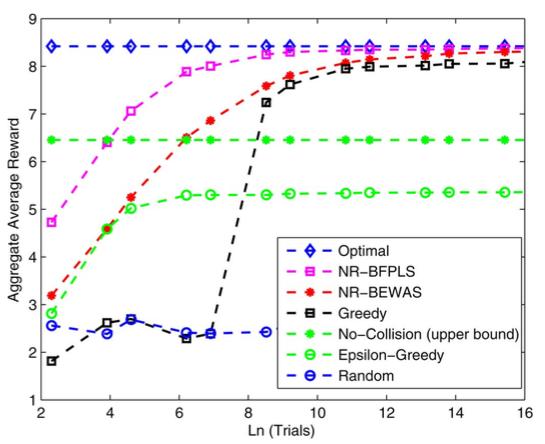
\epsfig{file=images/results_bandits_d2d.png, width=5cm}
					\caption{Average regret experienced by each of the action selection algorithms}
					\label{fig:bandits_results_d2d}
				\end{figure}
			

				In \cite{jamil2016novel} it is presented a centralized solution to adapt the transmission power and the carrier sense threshold of all the devices in a wireless network, with the aim of enhancing the spatial reuse while keeping a fair distribution of the average throughput. For that purpose it is used an Artificial Neural Network (ANN) with three layers (the input layer, one hidden layer, and the output layer). The number of inputs is two times the number $k$ of nodes to be manipulated, as well as each input represents the chosen value by each node for TPC and CCA parameters. The output in this case represents the throughput experienced by each node, so there are just $k$ neurons. 	
				\begin{figure}[h!]
					\centering
					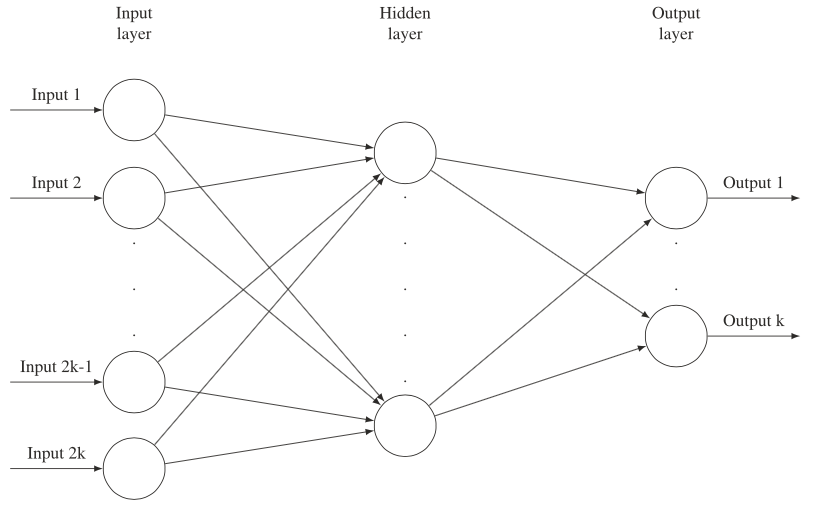
\epsfig{file=images/neural_network_topology.png, width=8cm}
					\caption{Topology of the ANN}
					\label{fig:neural_network_topology}
				\end{figure}	
				Since the main goal is to enhance the fairness experienced at the network as a whole, the following minimization function is used:
				\begin{equation}
					Cost_{fairness} = 1 - \frac{(\sum_{i=1}^{K}x_i)^2}{K\sum_{i=1}^{K}x_i^2}
				\end{equation}		
				In addition, it is sought to guarantee a minimum throughput $X_T$, so the following expression is also attempted to be minimized:
				\begin{equation}
					Cost_T = \sum_{i=1}^{K} \frac{(X_T - x_i)^2}{X_T}
				\end{equation}	
				Thus, the final cost used to evaluate the performance of the ANN is given by:
				\begin{equation}
					Cost_{tot} = Cost_{fairness}  + 1 \frac{1}{\sum_{i=1}^{K}X_T} \cdot Cost_T 
				\end{equation}	
				
				In the work it is also described the processes of data collection, training, testing and optimization, as well as the update phase. Basically, information for training/testing is constantly being updated to run the optimization, which error results are backpropagated to the previous levels. In case that the MSE (Mean Squared Error) and the desired fail number ratio ($\text{FNr}_{des}$) are below the expected results, the changes are applied and the process ends. Otherwise, both MSE and learning rate $\mu$ are decreased before running a new iteration (or epoch) of the whole process.
				
				\begin{figure}[h!]
					\centering
					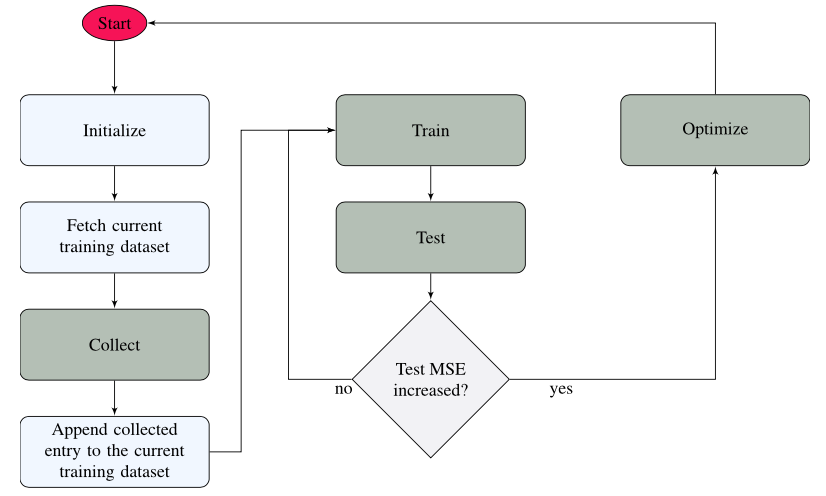
\epsfig{file=images/entire_procedure_ANN.png, width=10cm}
					\caption{Overall flow of the proposed ANN utilizations}
					\label{fig:entire_procedure_ANN}
				\end{figure}
				
				The results of using the ANN to adjust both TPC and CCA in a centralized manner, are shown at three different scenarios created at the OPNET simulator: exposed-node and hidden-node situations, and a high-density cellular scenario composed by 7 APs and 8 STAs per AP (the same scenario as for the mechanism revisited in Section \ref{section:cca_tpc_adaptation_fairness}). In all the cases, both aggregate throughput and fairness are enhanced after few epochs. In the high-density case, the gain noticed in the aggregate throughput exceeds the 45\%, while fairness starts from 0.5 and ends up to 0.7.

				\textcolor{red}{TODO: Table 4: learning in WNs}
				\begin{table}[h!]
					\centering
					\begin{tabular}{|l|l|l|l|l|}
						\hline
						\textbf{Work} & \textbf{Main Purpose} & \textbf{Centralised / Decentralised} & \textbf{Benefits} & \textbf{Drawbacks} \\ \hline
						{[}1{]} &  &  &  &  \\ \hline
						{[}2{]} &  &  &  &  \\ \hline
						{[}3{]} &  &  &  &  \\ \hline
					\end{tabular}
					\caption{Reinforcement Learning in WNs State-of-the-Art}
					\label{tbl:rl_wns}
				\end{table}			
	
	%%%%%%%%%%%%%%%%%%%%%%%%%%%%%%%%%%%%%%%
	% ONGOING WORK			        					   %%%%%%%%%%%%%
	%%%%%%%%%%%%%%%%%%%%%%%%%%%%%%%%%%%%%%%	
	\chapter{Current Contributions and Ongoing Work}
	\label{section:contributions}
	
		In this Section we describe the current contributions done, as well as the ongoing research tasks.

		\section{Wireless Networking Through Learning}
		\label{section:mdm}		
			Through the \textit{Wireless Networking Through Learning} project, which is under the Mar\'ia de Maeztu excellence program, the following contributions have been done:
			\begin{itemize}
				\item Conference paper submitted to the IEEE International Symposium on Personal, Indoor and Mobile Radio Communications (PIMRC) \cite{wilhelmi2017implications}.
				\item Journal article submitted to ...\textcolor{red}{TODO} \cite{wilhelmi2017enhancing}.
				\item Journal article in construction together with the Artificial Intelligence and Machine-Learning Research Group (AI-ML) \cite{bellalta2017learning}.
				\item Participation in the PhD Doctoral Workshop \cite{wilhelmi2017improving}.
				\item Collaboration in a Journal article in construction \cite{barrachina2017ctmn}.
				\item Inference of the coexistent devices configurations for allowing intelligent self-adjustment in dense WNs. This work is intended to be the result of a collaboration with the Wireless Communications department at Universidad Aut\'onoma Nacional de M\'exico (UNAM).
				\item Extension of \cite{wilhelmi2017enhancing} and \cite{wilhelmi2017implications} for exploring centralized approaches.
			\end{itemize}	
			
		\section{Other Projects}
		\label{section:other_projects}	
			\subsection{Analytical Models and Simulators}
			\label{section:validation}	
				In addition to the projects directly related to the main research activity, a fundamental task for this Thesis is to properly understand and/or develop the required simulation tools, which will allow us validating the results obtained from the research activity. One of the most important analytical model to compute the throughput in an overlapping network is the Continuous Time Markov Networks (CTMN) model \cite{bellalta2014throughput}, which captures the operation of the CSMA/CA protocol. In relation to this, we have started a collaboration for building a CTMN framework that builds the Markov chains according to the nodes input, which is leaded by Sergio Barrachina \cite{barrachina2017ctmn}. 
				
				Regarding simulators, we highlight ns-3, which is widely spread in the wireless community. However, the learning curve is high and many novel features are not yet supported. Since implementing them is a complex and time-consuming task, we are also building the Komondor simulator\footnote{\url{https://github.com/wn-upf/Komondor}}, as a result of a CISCO-UPF collaboration (further described in Section described in Section \ref{section:cisco_project}). Moreover, we are also interested in the Bianchi's model \cite{bianchi2000performance} for throughput computation in overlapping WLANs. The Bianchi's model is a benchmark in the current literature that we aim to use for validating the Komondor simulator.	

			\subsection{Development of an IEEE 802.11ax Event-Based Simulator}
			\label{section:cisco_project}	
				In order to perform simulations based on the IEEE 802.11ax standard, we have started building our own event-based simulator for WLANs, which has been called Komondor \cite{barrachina2017komondor}. Besides being a useful tool for supporting most of the research activity performed along the Thesis, the Komondor simulator is also the result of a collaboration with Cisco. Komondor is built on top of COST \cite{chen2005sense}, which provides the baseline for synchronised messages exchanging. The decision of building a simulator, apart from the Cisco's collaboration, lies in the impediments shown by other simulators like Network Simulator 3 (ns-3), which does not include many of the novel features provided by the IEEE 802.11ax standard, and which are the main matter of this Thesis. Moreover, building these functionalities in ns-3 is a extremely costly task, not only because of the complexity of the program, but for the significant learning curve.
				
				At the present time, Komondor v1.0 has been released and successfully validated against the well-known Bianchi's model for overlapping WLANs. Its main features are the Request to Send / Clear to Send (RTS/CTS) IEEE 802.11 mechanism, CSMA/CA with exponential slotted binary backoff (BEB), configurable packet traffic generation, collision type identification through logical events, and detailed statistics for metrics of interest such as average throughput per WLAN or detected hidden nodes. 			
				
			\subsection{AP Association and Self-Managed Networks through Learning}
			\label{section:fon_project}	
				We are also expected to contribute in the collaboration Fon-UPF, which is based in two main projects for improving network performance in coexistent wireless scenarios. Fon is a company that has built the world's largest network made up of people sharing their Wi-Fi. Due to new requirements in wireless networks and the increasing density in their main deployment scenario (residential buildings), Fon aims to enhance the AP association and autonomous management processes through Machine Learning techniques. For the former, a mobile application provided to users is used to gather information about the surrounding Fon networks, which is sent to a central unit. The latter must decide which is the best network for making user association.
				
				Secondly, to further improve network performance, an autonomous system for management is aimed to be provided. In this case, the gathered information for decision-making is also retrieved from the APs. The core idea is to empower the system with the necessary intelligence to allow self-adjustment in the Wi-Fi networks, so that the interference can be minimised along the network.
			
		\section{Preliminary Results}
		\label{section:preliminary_results}	
			The preliminary results obtained during the first year are focused on understanding network interactions, as well as to open discussion about the usage of RL in WNs. In \cite{wilhelmi2017implications}, we saw applying Q-learning in a decentralised manner to the resource allocation problem in dense WNs allows finding the best-performing actions that enhance the aggregate throughput. However, there is high variability in the throughput experienced by the individual networks. We identified the cause of this variability as the adversarial setting of our setup, in which the most played actions provide intermittent good/poor performance depending on the neighbouring decisions. An extension of \cite{wilhelmi2017implications} is provided in \cite{wilhelmi2017enhancing}, in which several Multi-Armed Bandits techniques are compared to solve the decentralised resource allocation problem in dense WNs. Each of the Bandits variations is extensively analysed to study the actual role of each of their parameters into networks performance and interactions.

	%%%%%%%%%%%%%%%%%%%%%%%%%%%%%%%%%%%%%%%
	% FUTURE WORK										   %%%%%%%%%%%%%
	%%%%%%%%%%%%%%%%%%%%%%%%%%%%%%%%%%%%%%%	
	\chapter{Planning and Future Work}
	\label{section:future_work}

		We have put forward a range of objectives to be accomplished during the development of the research activities related to this Thesis, which are listed below together with the involved tasks:
		\begin{itemize}
			\item \textbf{Objective 1 (O1):} Understanding the dynamics of coexistent WNs when competing for bandwidth resources.
			\begin{itemize}
				\item Extension of the current work in decentralised learning implications (DL1): Application of CTMN Framework to the work presented in \cite{wilhelmi2017implications}. Extend it to provide the centralised perspective.
			\end{itemize}
			\item \textbf{Objective 2 (O2):} Obtaining an extensive knowledge on the current techniques used for improving the spatial reuse in wireless networks.
			\begin{itemize}
				\item Make a publication collecting these techniques to provide an State-of-the-Art to the resource allocation problem in wireless networks (SOA1).
			\end{itemize}
			\item \textbf{Objective 3 (O3):} Understanding analytical and simulation tools for WNs performance computation.
			\begin{itemize}
				\item Komondor simulator: launch versions 2.1 (KM1) and 2.2 (KM2) that include intelligent agents to boost the network performance. Also, write a technical report to be published (KM3).
				\item CTMN framework collaboration with Barrachina: provide a framework to compute network throughput through the CTMN model (CTMN1).
			\end{itemize}
			\item \textbf{Objective 4 (O4):} Studying channel estimation and inference techniques to devise the behaviour of an overlapping WN from a decentralised point of view.
			\begin{itemize}
				\item Internship in Mexico (UNAM): Reinforcement Learning with Neighbouring Performance Inference for Resource Allocation in High-Density WLANs (UN1).
			\end{itemize}		
			\item \textbf{Objective 5 (O5):} Understanding the RL techniques, as well as Game Theoretical and Adversarial settings basics, that better suit the resource allocation problem in WNs. 
			\begin{itemize}
				\item Make a publication reviewing several techniques to prove their efficiency when applied in the wireless communications field (RL1).
			\end{itemize}		
			\item \textbf{Objective 6 (O6):} Understanding network dynamics and future requirements for dense wireless networks.
			\begin{itemize}
				\item Extrapolate the work done regarding RL in WNs in order to capture dynamics in terms of user and traffic variability (RL2). 
			\end{itemize}		
			\item \textbf{Objective 7 (O7):} Providing ML-based solutions to the resource allocation problem in future WLANs.
			\begin{itemize}
				\item Make a publication summarizing all the work done during the Thesis, which provides a ML-based solution to the resource allocation problem in future WLANs (ML1).
			\end{itemize}		
		\end{itemize}
	
		In parallel, and for the proper development of other, we define a set of objectives that differ from the main research line of this Thesis, but which provide complementary knowledge and enrich the degree of expertise in other fields.
		\begin{itemize}
			\item \textbf{Extra Objective 1 (EO1): FON collaboration} 
			\begin{itemize}
				\item Acquire the necessary knowledge to face the AP association problem in WNs from both decentralised and centralised perspectives. Thus, provide a State-of-the-Art in the field (FON1).
				\item Acquire the necessary knowledge for self-adjustment in WNs Thus, provide a State-of-the-Art in the field (FON2).
			\end{itemize}
			\item \textbf{Extra Objective 2 (EO2): Cisco collaboration} 
			\begin{itemize}
				\item Provide a wireless networks simulator that includes novel features in IEEE 802.11ax (CISCO1).
			\end{itemize}
		\end{itemize}
	
		The Gantt diagram below places the aforementioned tasks to be done along the next two years:	
	
		\noindent\resizebox{\textwidth}{!}{
			\begin{tikzpicture}[x=.5cm, y=1cm]
				\begin{ganttchart}[vgrid,hgrid]{1}{24}
					\gantttitle{2017}{3} \gantttitle{2018}{12} \gantttitle{2019}{9}\\
					\gantttitlelist{10,...,12}{1} \gantttitlelist{1,...,12}{1} \gantttitlelist{1,...,9}{1} \\
					% 
					\ganttgroup{O1}{1}{5} \\
					\ganttmilestone{DL1}{5} \ganttnewline
					% 
					\ganttgroup{O2}{1}{8} \\
					\ganttmilestone{SOA1}{2} \ganttnewline
					%
					\ganttgroup{O3}{1}{8} \\
					\ganttmilestone{KM1}{2} \ganttnewline
					\ganttmilestone{KM2}{8} \ganttnewline
					\ganttmilestone{KM3}{3} \ganttnewline
					\ganttmilestone{CTMN1}{5} \ganttnewline				
					% 
					\ganttgroup{O4}{3}{8} \\
					\ganttmilestone{UN1}{8} \ganttnewline
					% 
					\ganttgroup{O5}{9}{10} \\
					\ganttmilestone{RL1}{10} \ganttnewline
					%
					\ganttgroup{O6}{9}{10} \\
					\ganttmilestone{RL2}{10} \ganttnewline
					%			
					\ganttgroup{O7}{9}{10} \\
					\ganttmilestone{ML1}{10} \ganttnewline
					%
					\ganttgroup{EO1}{9}{10} \\
					\ganttmilestone{FON1}{10} \ganttnewline
					\ganttmilestone{FON2}{10} \ganttnewline
					%
					\ganttgroup{EO2}{9}{10} \\
					\ganttmilestone{CISCO1}{10} \ganttnewline
				\end{ganttchart}
			\end{tikzpicture}
		}	
	
	%%%%%%%%%%%%%%%%%%%%%%%%%%%%%%%%%%%%%%%
	% BIBLIOGRAPHY					      				   %%%%%%%%%%%%%
	%%%%%%%%%%%%%%%%%%%%%%%%%%%%%%%%%%%%%%%	
	\bibliographystyle{unsrt}
	\bibliography{bib}

\end{document}